\documentclass[12pt]{article}
\usepackage[utf8]{inputenc}
\usepackage{chapterbib}
\usepackage[sectionbib,numbers]{natbib}
\usepackage{eurosym}
\usepackage{amstext,amsthm}
\usepackage{amsmath}
\usepackage{amssymb,mathtools}
\usepackage[nointegrals]{wasysym} % enthaelt iint-Def die aber auch in amsmath definiert sind
\usepackage{mathrsfs}
\usepackage{hyperref}
%\usepackage{refcheck}
\usepackage{graphicx}
\usepackage[figuresleft]{rotating}

\usepackage{tikz}
%\usepackage{enumerate}

\newtheorem{proposition}{Proposition}[section]
\newtheorem{corollary}[proposition]{Corollary}
\newtheorem{theorem}{Theorem}
\newtheorem{lemma}{Lemma}[section]
\theoremstyle{definition}
\newtheorem{definition}{Definition}[section]
\newtheorem{remark}{Remark}[section]
\newtheorem{example}{Example}[section]
\newtheorem{estimator}{Estimator}[section]
\pagestyle{headings}

\setlength{\bibsep}{0pt}

\setlength{\textheight}{230mm}
\setlength{\topmargin}{-15mm} 
\setlength{\textwidth}{17cm} 
\setlength{\oddsidemargin}{-3mm}
\setlength{\columnseprule}{.1pt}
\setlength{\columnsep}{20pt}

\def\blstr{1.1}
\renewcommand{\baselinestretch}{\blstr}
\def\blstrtable{1.55}
\def\blstrcode{1.2}  
%\renewcommand{\labelenumi}{\alph{enumi})}
%%\setlength{\oddsidemargin}{0.28in} 
%%\setlength{\evensidemargin}{0.28in}

\addtolength{\bibsep}{1.5mm}
%%\bibpunct{(}{)}{,}{a}{}{,}

%%\RequirePackage{ae,mathpple}
%%\renewcommand{\rmdefault}{ppl}
%%\renewcommand{\sfdefault}{aess}
%%\renewcommand{\ttdefault}{aett}
\newcommand{\Rpackage}[1]{{\normalfont\fontseries{b}\selectfont #1}}

%\usepackage{a4}
\usepackage[normalem]{ulem}
\usepackage{color}
\newcommand{\dirk}[3]{\textcolor{red}{\sout{#1}\textcolor{blue}{#2}}{\begin{marginpar}{\raggedright\color{red} Dirk:\tiny {#3}}\end{marginpar}}}
\newcommand{\peter}[3]{\textcolor{red}{\sout{#1}\textcolor{blue}{#2}}{\begin{marginpar}{\raggedright\color{green} Peter:\tiny {#3}}\end{marginpar}}}


\DeclareMathAlphabet{\mathpzc}{OT1}{pzc}{m}{it}
\newcommand{\smallu}{\mathpzc{u}}
\newcommand{\smallx}{\mathpzc{x}}
\newcommand{\smally}{\mathpzc{y}}
\newcommand{\smallz}{\mathpzc{z}}
\newcommand{\ind}[1]{\mathbbm{1}_{\{#1\}}} %Definition Indikatorfunktion
\newcommand{\indset}[1]{\mathbbm{1}_{#1}} %Definition Indikatorfunktion
\providecommand{\abs}[1]{\lvert#1\rvert}
\providecommand{\norm}[1]{\lVert#1\rVert}


\usepackage{times}
%%\RequirePackage[T1]{fontenc}

\begin{document}
\title{\LARGE Inference of recent admixture using genotype data}

\author{\sc Peter Pfaffelhuber, Elisabeth Huss, Denise
  Syndercombe Court, \\ \sc Franz Baumdicker, Fabian Staubach}

\date{\today}

\maketitle

FROG-kB




\begin{abstract}
  For inference of individual genetic histories, admixture barplots
  are being used abundantly in forensic genetics. The underlying
  admixture-model (as e.g.\ implemented in the software {\sc
    structure} and {\sc admixture}) assumes parameters for individual
  ancestry (IA). Further, every allele in the individual's genome
  originates in one of several ancestral populations with the same
  probability. Here, we introduce the recent-admixture model. In this
  model, we assume that the two homologous copies of each allele
  originate from the ancestral populations independently for the
  mother's and the father's copy. Estimates for IA in absence of
  recent admixture are almost identical for the admixture and recent
  admixture model. However, they are more accurate for the
  recent-admixture model in individuals which are in fact recently
  admixed.  Moreover, we develop a likelihood ratio test for recent
  admixture, which has a high power to find recently admixed
  individuals. We analyse data from the 1000 genomes dataset with our
  methods and find some recently admixed individuals.
\end{abstract}

\section{Introduction}
xxx Start with forensics

xxx Make a good case, e.g. Philippino and Italian located in
Afghanistan

Inference of the geographical ancestry of a trace using genetic
markers is today a well-established research field in forensic
genetics (see e.g.\ \cite{Phillips2016, Eduardoff2016,
  Kidd2017}). Either the trace is classified into one of several
groups of different origin (e.g.\ Africa, Europe, East Asia, Native
America, and Oceania; see e.g.\ \cite{Snipper2007, Pfaffelhuber2019},
or it is assumed that it consists of a mixture of ancestral genetic
material originating in several groups. For this task, {\sc structure}
\cite{Pritchard2000} has become the de-facto standard to estimate
individual ancestry (IA) proportions of a trace among several
continental groups. (This Bayesian approach using MCMC was
complemented by the faster, likelihood based approach, implemented in
the software {\sc admixture} \cite{Alexander2009}; see also
\cite{Tang2005} for the same model.).

When using {\sc structure} or {\sc admixture} for estimating
continental (or other scales of geography) IA of a trace, allelic
frequencies for all continents from a reference database must be
used. A main assumption for estimating IAs is that all allelic states
have the same independent chance to share a copy from some continent,
implying Hardy-Weinberg equilibrium at each site. When using a (small)
set of ancestry informative markers, this assumption is justified by
the large genomic distance which makes loci almost independent by
recombination. However, the assumption that homologous alleles at the
same locus have the same probability for carrying some allele -- also
known as Hardy-Weinberg equilibrium -- may not always hold. For
example, consider an individual whose parents have different
continental backgrounds, and an allele which separates perfectly
between the two continents. Then, the individual will certainly be a
heterozygote at this marker.  This increase in frequency for
heterozygotes under admixture is known for a long time and usually
called the Wahlund effect \cite{Wahlund1928}.  However, {\sc
  structure} and {\sc admixture} will estimate that the chance for
some allele to come from one of the two continents to be 50\%, which
is then also be the estimate for a heterozygote at the locus (due to
the assumption of independence of allelic states in the admixture
model).

Inference of recent admixture is often based on an excess of
heterozygotes. For example, \cite{McNevin2019} uses a statistical test
by simply counting the number of heterozygous positions in an
individual in order to infer recent admixture. Extending work of
\cite{Tvedebrink2018a}, a likelihood-ratio test for first-order admixed
individuals versus outside-of-reference-database is given in
\cite{Tvedebrink2019}. Here, we extend the likelihood-model behind
{\sc structure} or {\sc admixture} in order to account for recent
admixture. In our approach, IA consists of two vectors, one for each
parent. As a result, we obtain estimates of IA for the two parents and
can give a likelihood ratio test for recent admixture versus
non-admixture of a trace.

xxx some more detail for our approach

xxx Mention Tvedebrink2019, Cheung2018.

xxx Tvedebrink assigns first generation admixed individuals wrongly to admixed populations (FS)

xxx explain exchangeability of $q^M, q^P$.

xxx $p$-value when our error is better (admixture, recent-admixture);

xxx Figure in Supplement: AFR, EAS, EUR, SAS not worse in
recent-admixture



\section{Materials and Methods}
\sloppy More details on the derivations in the admixture and
recent-admiture model can be found in the SI. Moreover, the
implementation of our methods can be downloaded from \url{
  https://github.com/pfaffelh/recent-admixture}, and is described in
detail in the SI.

\subsection{The admixture model}
We briefly recall the admixture model, which is the basis for the
sofware {\sc structure} \cite{Pritchard2000}, {\sc admixture}
\cite{Alexander2009} and {\sc frappe} \cite{Tang2005}.  Here and
below, we assume to have reference database of $M$ bi-allelic markers
from $K$ populations. We denote by $p_{mk}$ the frequency of allele~1
at marker $m$ in population $k$. We have a trace with
$G_m \in \{0,1,2\}$ copies of allele~1 at marker $m$ for
$m=1,...,M$. Assuming that each allele observed in the trace comes
from population $k$ with probability $q_k$, the probability to observe
allele~1 at marker $m$ is
\begin{align}
  \label{eq:beta}
  \beta_m(q) := \sum_k p_{mk} q_k,  
\end{align}
and the log-likelihood of $q = (q_k)_{k=1,...,K}$ is (see also~(S1) in
the SI)
\begin{align}\label{eq:logLadmixture}
  \ell(q|G) = \sum_{m=1}^M \log\Big(\binom{2}{G_m} \beta_m(q)^{G_m}(1-\beta_m(q))^{2-G_m}\Big).
\end{align}
Assuming that all $p_{mk}$'s are known, this function can be maximized
over $q$ by computing $\hat q = (\hat q_k)_{k=1,...,K}$ such that
$\hat q_k = f_k(\hat q)$ for (see also \eqref{eqSI:fixed} in the SI)
\begin{align}\label{eq:fixed}
  f_k(q) =
  \frac{1}{2M} \sum_{m=1}^M \Big(G_m \frac{p_{mk}}{\beta_m(q)} + (2-G_m)\frac{1-p_{mk}}{1-\beta_m(q)}\Big)q_k,
  \qquad k =1,...,K.
\end{align}
This can be done numerically by iterating
$q_{n+1} = (f_k(q_n))_{k=1,...,K}$ until convergence. (In our
implementation, we continue the iteration until
$|q_{n+1} - q_n|< 10^{-6}$.) We note that this approach is essentially
the same as in the EM-algorithm from \cite{Tang2005}, but combining
the expectation and maximization steps. In addition, although
maximizing \eqref{eq:logLadmixture} could also be handled using a
Newton method as in \cite{Alexander2006}, this approach has the
advantage that $q_n$'s are positive in all steps, and the sum of all
entries in $q_n$ is always~1. Moreover, the iteration is
computationally fast if only a small or moderat number of alleles is
considered.

\subsection{The recent-admixture model}
When mother and father of an individual come with their own vectors of
admixture proportions, $q^M$ and $q^P$, the log-likelihood from
\eqref{eq:logLadmixture} changes to (see also
\eqref{eqSI:logLrecentadmixture} in the SI)
\begin{align}\label{eq:logLrecentadmixture}
  \ell(q^M, q^P|G) & = \sum_{m=1}^M \log( \gamma_m(q^M, q^P, G_m)),
  \\
  \notag
  \gamma_m(q^M, q^P, g) & = \begin{cases}\beta_m(q^M) \beta_m(q^P), & \text{ if }g=2,\\
    (\beta_m(q^M) (1-\beta_m(q^P))
    + (1-\beta_m(q^M)) \beta_m(q^P)), & \text{ if }g=1,\\
    (1-\beta_m(q^M))(1-\beta_m(q^P)), & \text{ if }g=0. \end{cases}
\end{align}
\sloppy As carried out in the SI, this function can be maximized by
computing $\hat q^M, \hat q^P$ such that
$\hat q^P = f(\hat q^M, \hat q^P)$ and
$\hat q^M = f(\hat q^P, \hat q^M)$ for
$f(q,q') = (f_k(q, q'))_{k=1,...,K}$ with (see
\eqref{eqSI:fixedRecent} in the SI)
\begin{align}\label{eq:fixedRecent}
  f_k(q, q') & := \frac{1}{M}\sum_{m=1}^M \delta_k(q,q', G_m) q_k',
  \\
  \notag
  \delta_k(q^M, q^P, g) & = \begin{cases}
    \displaystyle\frac{p_{mk}}{\beta_m(q')}, & \text{ if }g=2,\\[2ex]
    \displaystyle\frac{(p_{mk} (1-\beta_m(q))
      + (1-p_{mk})\beta_m(q))}{\beta_m(q)(1-\beta_m(q'))
      + (1-\beta_m(q))\beta_m(q')}, & \text{ if }g=1,\\[2ex]
    \displaystyle\frac{(1-p_{mk})}{1-\beta_m(q')}, & \text{ if }g=0. \end{cases}
\end{align}
In our implementation, we iteratively compute
$q_{n+1}^F = f(q_n^M, q_n^F)$ and
$q_{n+1}^M = f(\tilde q_{n+1}^F, q_n^M)$ until convergence.

\subsection{Obtaining admixed individuals in silico}
\label{S:insilico}
In order to test our method, we created admixed individuals from a
reference database. (We use the 1000 genomes dataset, but excluding
Admixed Americans, AMR; see below.) For example, we obtain an
individual admixed from populations $k$ and $k'$ by choosing a genome
$\tilde G = (\tilde G_m)_{m=1,...,M}$ from population $k$ and
$\bar G = (\bar G_m)_{m=1,...,M}$ from population $k'$ as the
parents. Then, $G_m = X_m + Y_m$ where $X_m = 1$ with probability
$\tilde G_m/2$, $X_m=0$ with probability $(2-\tilde G_m)/2$ and
$Y_m = 1$ with probability $\bar G_m/2$, $Y_m=0$ with probability
$(2-\bar G_m)/2$. When iterating this procedure, we can also model
second-order admixed individuals etc.\ in silico.

Using AFR, EAS, EUR, SAS as population labels (as in the 1000 genomes
dataset), all cases for second generation admixed individuals fall
into one of seven categories. Writing up the ancestries of the four
grand-parents (Mother of mother, father of mother / mother of father,
father of father), we have the following cases for second generation
admixed individuals (the full list of all resulting 55 cases is given
in the SI; note that \cite{Cheung2018} come up with only 35 cases,
since they do not distinguish between maternal and paternal ancestry,
e.g.\ they count AFR, AFR / EAS, EAS and AFR, EAS / AFR, EAS as one
case):

\begin{itemize}
\item[(A)] 4 non-admixed cases, e.g.\ AFR, AFR/ AFR, AFR;
\item[(B)] 6 admixed cases with admixture ratio 50:50, where both
  parents are non-admixed, e.g. AFR, AFR/ EAS, EAS;
\item[(C)] 6 admixed cases with admixture ratio 50:50, where both
  parents are admixed, e.g.\ AFR, EAS/ AFR, EAS;
\item[(D)] 12 admixed cases with admixture ratio 75:25, e.g.\ AFR,
  AFR/ AFR, EAS;
\item[(E)] 12 admixed cases with admixture ratio 50:25:25, where one
  parent is non-admixed, e.g.\ AFR, AFR/ EAS, EUR;
\item[(F)] 12 admixed with admixture ratio 50:25:25, where both
  parents are admixed, e.g.\ AFR, EAS/ AFR, EUR;
\item[(G)] 3 admixed with admixture ratio 25:25:25:25, e.g.\ AFR, EAS/
  EUR, SAS;
\end{itemize}
For each of the other 55 cases, we simulated 500 individuals in silico
by picking four grand-parents at random from the populations, creating
mother and father from the grand-parents, and creating a new
individual from the parents, as described above.

\subsection{Comparing results from admixture and recent-admixture}
For a reference database from which we compute (or estimate) allele
frequencies $p_{mk}$ (which is the allele frequency of allele~1 at
marker $m$ in population $k$), we can estimate $q$ from the admixture
model as well as $q^M,q^P$ from the recent-admixture model, as
described in \eqref{eq:fixed} and \eqref{eq:fixedRecent}. In order to
compare the results from the admixture and recent-admixture model, we
compute $q_k^{MF} := \tfrac 12 (q_k^M + q_k^F)$ for $k=1,...,K$, which
give the fractions of the genome coming from populations
$1,...,K$. Then, for a non-admixed individual, we have
$q_k^{\text{\sc true}} = 1$ for some $k$, and for an admixed
individual with parents from populations $k$ and $k'$ we have
$q_k^{\text{\sc true}} =q_{k'}^{\text{\sc true}} = 0.5$, and similarly
for individuals with grandparents from three or four different
populations. Computing the estimation error, i.e.\ the distance to the
true IA for the admixture model, results in
\begin{align}
  \label{eq:error}
  \sum_k |q_k - q_k^{\text{\sc true}}| \text{  and }\sum_k |q_k^{MF} - q_k^{\text{\sc true}}|
\end{align}
for the recent-admixture model. We stress that in the recent-admixture
model, we in fact obtain results for $q^M$ and $q^P$ separately, such
that even more information than $q^{MF}$ is contained in the estimates
for this model.

\subsection{A likelihood-ratio test for recent admixture}
We want to test if data $G = (G_m)_{m=1,...,M}$ from a new trace fits
significantly better to the recent-admixture model than to the
admixture model. Since the admixutre model is identical to the
recent-admixture model for $q^M = q^P = q$, we are testing the
hypothesis $H_0: q^M = q^P$ against $H_1: q^M\neq q^P$. For this, we
take the estimators $\hat q$ of $q$ from iteration of
\eqref{eq:fixed}, and $\hat q^M, \hat q^P$ of $q^M$ and $q^P$ from
iteration of \eqref{eq:fixedRecent} and compute
$\Delta\ell := \ell(\hat q^M, \hat q^P|G) - \ell(\hat q|G)$ with
$\ell(q^M, q^P|G)$ from \eqref{eq:logLrecentadmixture} and $\ell(q|G)$
from \eqref{eq:logLadmixture}. If $\Delta \ell >x$ for some $x$ (which
needs to be specified), the recent-admixture model fits significantly
better and we reject $H_0$. If $\Delta \ell \leq x$, we accept
$H_0$. In order to find $x$, we fix a $p$-value (1\%, say), and take
$x$ to be the $p$-quantile of the empirical distribution for data in
the reference database. (This means, if $p=1\%$ and the reference
dataset contains 1000 samples, we compute all values for $\Delta\ell$
for all samples, and set $x$ to be the 10th-smallest value we
obtained.)

\subsection{Human data}
\sloppy We downloaded 1000 Genomes data (phase 3) from
\url{ftp://ftp.1000genomes.ebi.ac.uk/vol1/ftp/release/20130502/}, as
well as information on the sampling locations from
\url{ftp://ftp.1000genomes.ebi.ac.uk/vol1/ftp/release/20130502/integrated_call_samples_v3.20130502.ALL.panel}
\cite{Auton2015}. This is data from 661 individuals from Africa (AFR),
347 Admixed Americans (AMR), 504 East Asians (EAS), 503 Europeans
(EUR) and 489 South-East Asians (SAS).

xxx Explain why we use EUROFORGEN, Kidd

The dataset comes with approximately 80 million SNPs.  However, we use
only a few of them known as the EUROFORGENE AIMset \cite{Phillips2014}
and Kidd AIMset \cite{Kidd2014}, respectively. The EUROFORGENE AIMset
comes with 128 SNPs able to distinguish between continental
groups. Here, we ignore tri-allelic SNPs (rs17287498, rs2069945,
rs2184030, rs433342, rs4540055, rs5030240), as well as rs12402499,
which is not available in the 1000 genomes dataset. The Kidd AIMset
consists of 55 bi-allelic SNPs, all of which are available in the 1000
genomes dataset.

\section{Results}

xxx compare runtimes

\subsection{Estimation accuracy}
Both, the admixture model and the recent-admixture model give
estimates of IA. Using data from the 1000 genomes, but excluding all
Admixed Americans (AMRs) since they are known to have an admixed
background \cite{Eduardoff2016, Pfaffelhuber2019}, we use the SNPs
from the EUROFORGENE and Kidd AIMsets. We use the continental origins
as described in the dataset, i.e.\ we have AFR (African), EAS
(East-Asia), EUR (European) and SAS (South-Asian) samples. As
described in MM, we average estimates $\hat q^M$ and $\hat q^P$ from
the recent-admixture model, in order to compare to the true IAs. As
can be seen in Figure~\ref{fig:mixed_cases}.A, the recent-admixture
estimates outperform admixture estimates in all cases (which were
created in silico as described in MM) for first generation admixed
individuals. For second generation admixed individuals, the situation
is similar, but depending on the type of admixture; see cases (B)--(G)
as defined in Section~\ref{S:insilico} above. (A full list of~55 cases
is displayed in Figure~\ref{fig:mixed_allcases} in the SI.) In
Figure~\ref{fig:mixed_cases}.B, note that column~A gives non-admixed
samples, and we see that estimates of IA are essentially as accurate
in the admixture model and the recent-admixture model. All results for
the Kidd AIMset are similar and found in the SI.

\begin{figure*}[htb]
  \hspace{3cm} (A) \hspace{8cm} (B)
  \begin{center}
    \parbox[b]{0.45\textwidth}{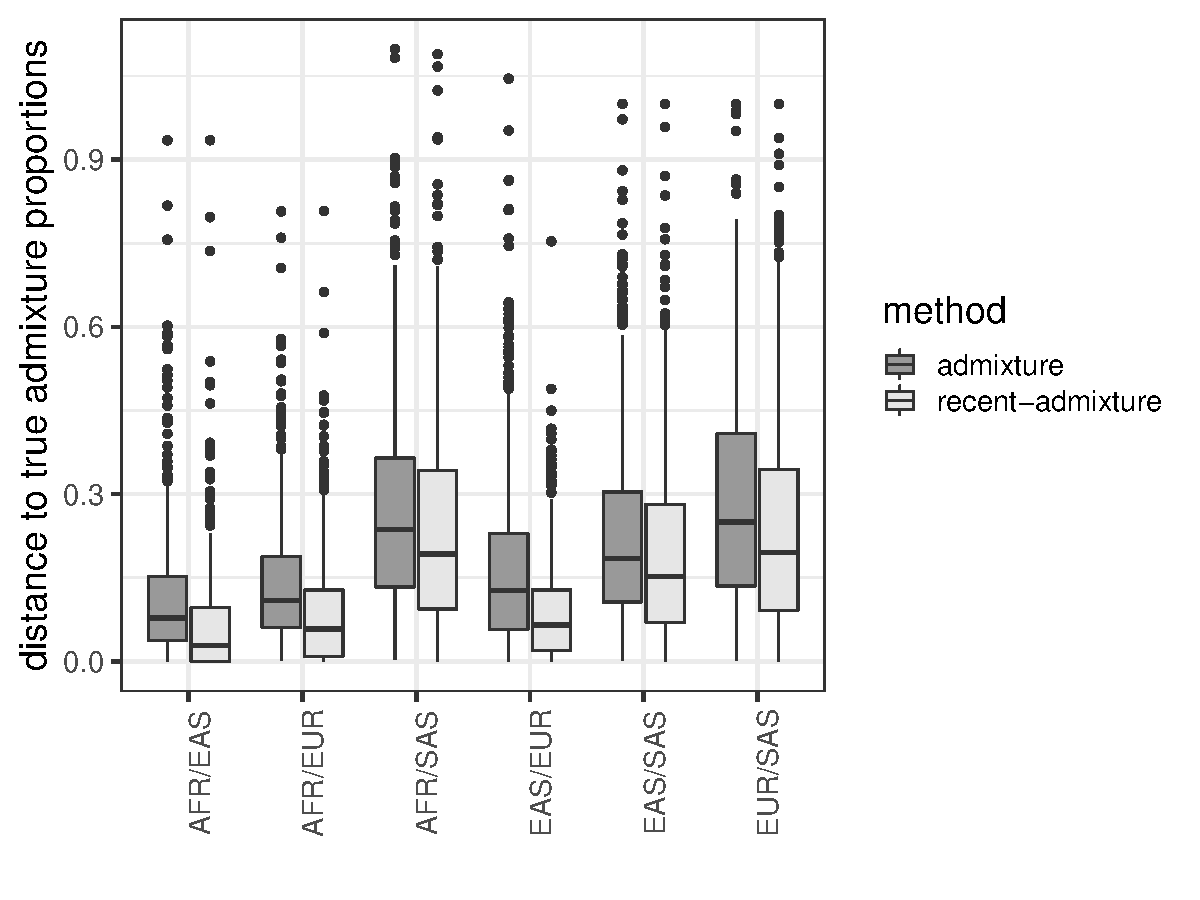
\includegraphics[width=0.45\textwidth]{deviations_mixed.pdf}\vspace{2cm}}
    \hspace{1cm}
    \parbox[b]{0.45\textwidth}{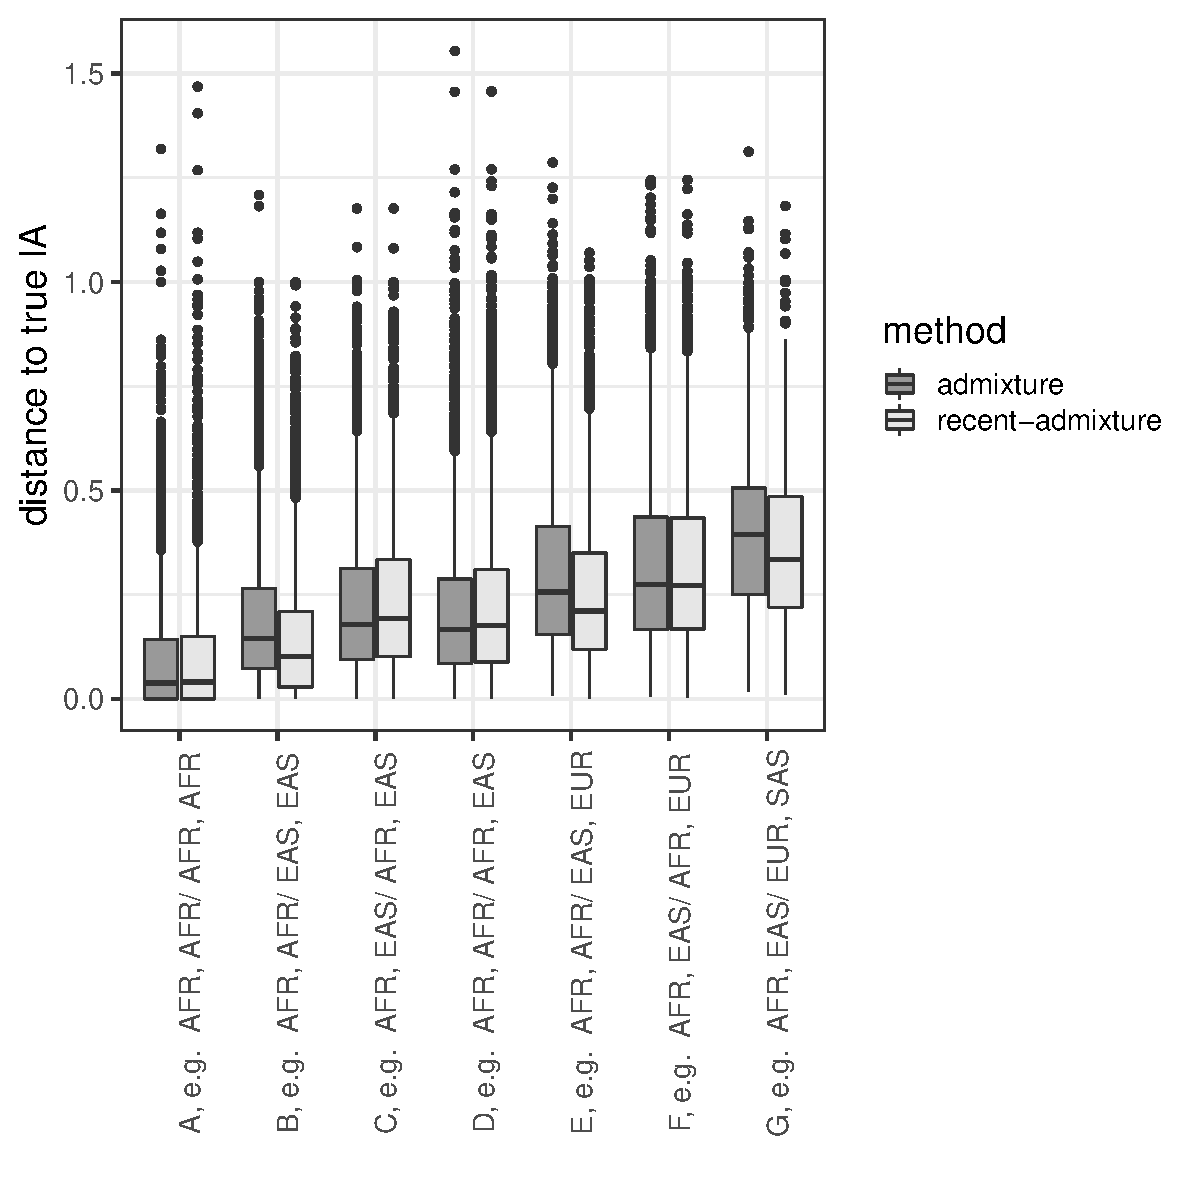
\includegraphics[width=0.45\textwidth]{deviations_mixed_cases.pdf}}
  \end{center}
  \caption{\label{fig:mixed_cases} For all first generation admixed
    samples (A) and second generation admixed samples (B), we computed
    IA from the admixture and recent-admixture model. The distance to
    the true IA is computed as in \eqref{eq:error}. The cases in (B)
    are as described above. xxx add $p$-values xxx put a figure for
    the non-admixed scenario in the SI.}
\end{figure*}

\subsection{Power of the Likelihood-ratio test for recent admixture}
When fixing the maximal $p$-value for significance of the
likelihood-ration test for recent admixture (as described in MM), we
obtain the power of the test for all cases of recent
admixture. Displaying the false positives (i.e.\ positively tested
non-admixed) against true positives (i.e.\ positively tested admixed)
in cases (B)--(G) for all possible values of $p$, we obtain the
Receiver-Operation-Characteristic (ROC) curve (xxx ref). The optimal
curve nearly hits~0 false positives with~100\% true positives and has
an AUC (Area Under the Curve) of~1. As we see in Figure~\ref{fig:ROC},
the power of the test differs with the kind of admixture. For first
generation admixed (case (B)), one non-admixed parent (case (E)) and
all grand-parents from different continents (case (G)), the test is
nearly perfect in distinguishing recent-admixture from admixture. If
only half of the genome has two different ancestries (cases (D) and
(F)), the power is reduced. If the individual is not recently-admixed
in first generation, but both parents are (case (C)), power drops even
more. In fact, the latter case is not recent-admixture as in our
definition, since $q^M = q^P$ should technically hold. For the overall
performance of the test, we give some examples in
Table~\ref{tab:power}, in particular the power at $p=1\%$ and AUC in
all cases. Results for the EUROFORGEN AIMset are marginalle better
than for the Kidd AIMset, which are given in the SI in
Figure~\ref{fig:ROC_Kidd} and Table~\ref{tab:power_Kidd}.

\begin{figure*}[htb]
  \begin{center}
    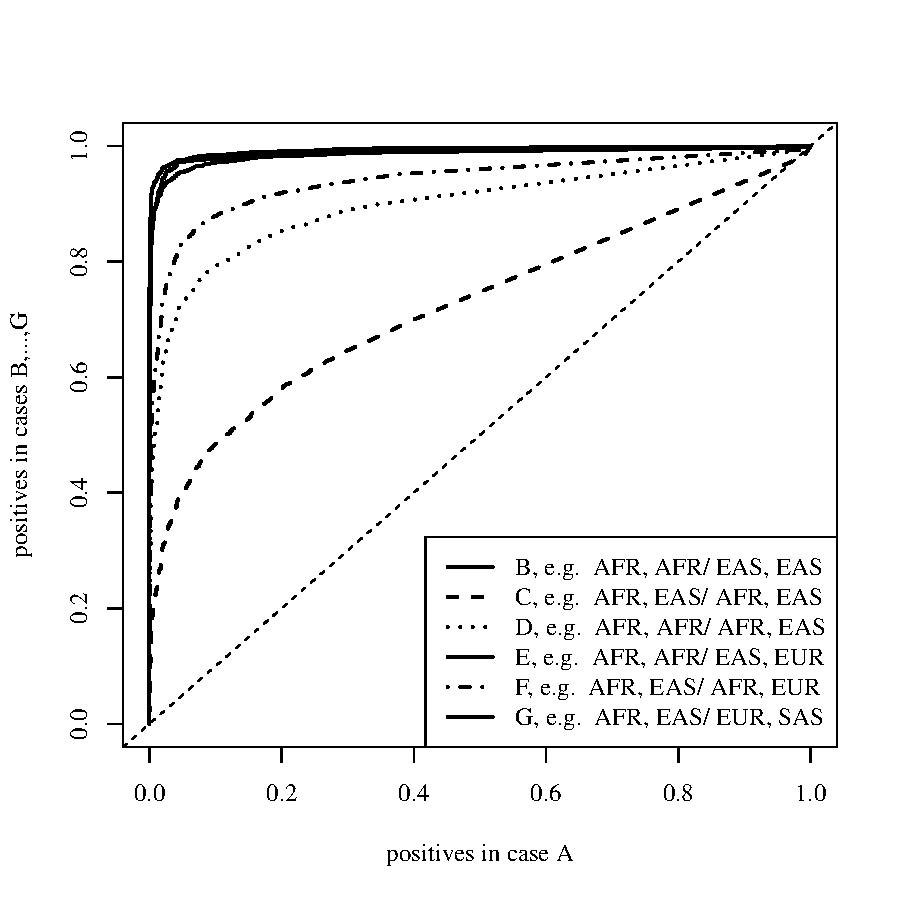
\includegraphics[width=0.45\textwidth]{roc-curve-EUROFORGENE.pdf}
  \end{center}
  \caption{Using the EUROFORGEN AIMset, we plot false positives (i.e.\
    positive non-admixed individuals, as in case (A) above, againts
    positives for all cases of admixture in second generation.}
  \label{fig:ROC} 
\end{figure*}

\begin{table}
  \centering
  \begin{tabular}{l|rrrrrr}
Case & B & C & D & E & F & G \\ \hline
AUC &  0.99  &  0.637  &  0.872  &  0.983  &  0.928  &  0.99 \\ Power at $p=0.01$ & 0.94  &  0.23  &  0.51  &  0.9  &  0.62  &  0.9 \\
 \end{tabular}

  \caption{Using the same data as in Figure~\ref{fig:ROC}, we e.g.\
    see that the test for recent admixture turns out to have a
    $p$-value below~1\% in 94\% cases of first generation admixed
    individuals. xxx add false positives to x-axis, add true positives
    to y-axis.}
  \label{tab:power}
\end{table}

xxx compare with Tvedebrink

\subsection{Recent admixture in the 1000 genomes dataset}
From the 1000 genomes dataset, we highlight individuals which give
significant results for the test of recent admixture for both
AIMsets. We exclude AMRs from our analysis, and give in
Table~\ref{fig:1000r-ad} the eight most extreme cases, which show
highly significant results for recent admixture for both
AIMsets. There are six Africans from population ASW (Americans from
Southwest USA), and two from South Asia, one from GIH (Gujarati Indian
from Houston, Texas) and one from BEB (Bengali from Bangladesh). We
note that it is known that the ASW population is admixed
\cite{Eduardoff2016}, but until now, it has not been tested if
admixture is recent.

\begin{itemize}
\item NA20278: Giving the most significant results for both datasets,
  this male has most probably parents of African and European
  ancestry. Note also that $q^{MF}$ and $q$ are very similar for both
  AIMsets.
\item NA20342, NA19625, NA20355: Clearly, one parent has African
  ancestry. The other parent is most likely partly European.
\item NA20274: Our test indicates two parents of different ancestry,
  one mostly African, the other mostly East-Asian.
\item NA20299: Interestingly, the results for both AIMsets differ in
  this example. One parent has most likely African ancestry, the other
  is European according to the EUROFORGEN AIMset and South-Asian
  according to the Kidd AIMset.
\item HG03803: Most likely, one parent is of South-Asian, the other
  has East-Esian ancestry.
\item NA20864: Most likely, one parent is of South-Asian, the other
  has European ancestry.
\end{itemize}

In order to get a clearer picture about {\em true} ancestries in these
individuals, we examined local ancestry in the genome. xxx


\newcommand\crule[3][black]{\textcolor{#1}{\rule{#2}{#3}}}
\begin{figure}[p]
  \parbox{.5\textwidth}{\begin{tabular}{ll|r}
\multicolumn{3}{l}{NA20278, AFR, ASW}\\ \hline\rule[-1ex]{0cm}{4ex}EURO & ad \hspace{1cm} \parbox{.5cm}{$q$ \\[-1.3ex] \mbox{}}& \begin{tikzpicture} 
\draw[fill=red] (0cm, 0cm) rectangle (0.916cm, .4cm);
\draw[fill=blue] (0.916cm, 0cm) rectangle (0.938cm, .4cm);
\draw[fill=green] (0.938cm, 0cm) rectangle (2cm, .4cm);
\draw[fill=yellow] (2cm, 0cm) rectangle (2cm, .4cm);
\end{tikzpicture}
\\ \cline{2-3}
\rule[-3ex]{0cm}{7ex} $\Delta\ell =$  6.69 & r-ad \hspace{0cm} \parbox{1cm}{\hfill $q^{MF}$ \ $q^M, q^F$} & \parbox{2cm}{\begin{tikzpicture} 
\draw[fill=red] (0cm, 0cm) rectangle (0.96cm, .4cm);
\draw[fill=blue] (0.96cm, 0cm) rectangle (1.014cm, .4cm);
\draw[fill=green] (1.014cm, 0cm) rectangle (2cm, .4cm);
\draw[fill=yellow] (2cm, 0cm) rectangle (2cm, .4cm);
\end{tikzpicture}
\\[-1.3ex]\begin{tikzpicture} 
\draw[fill=red] (0cm, 0cm) rectangle (1.894cm, .2cm);
\draw[fill=blue] (1.894cm, 0cm) rectangle (2cm, .2cm);
\draw[fill=green] (2cm, 0cm) rectangle (2cm, .2cm);
\draw[fill=yellow] (2cm, 0cm) rectangle (2cm, .2cm);
\end{tikzpicture}
\\[-2ex]\begin{tikzpicture} 
\draw[fill=red] (0cm, 0cm) rectangle (0.028cm, .2cm);
\draw[fill=blue] (0.028cm, 0cm) rectangle (0.028cm, .2cm);
\draw[fill=green] (0.028cm, 0cm) rectangle (2cm, .2cm);
\draw[fill=yellow] (2cm, 0cm) rectangle (2cm, .2cm);
\end{tikzpicture}
}\\ \hline 
\rule[-1ex]{0cm}{4ex}Kidd & ad \hspace{1cm} \parbox{.5cm}{$q$ \\[-1.3ex] \mbox{}}& \begin{tikzpicture} 
\draw[fill=red] (0cm, 0cm) rectangle (0.934cm, .4cm);
\draw[fill=blue] (0.934cm, 0cm) rectangle (0.954cm, .4cm);
\draw[fill=green] (0.954cm, 0cm) rectangle (1.948cm, .4cm);
\draw[fill=yellow] (1.948cm, 0cm) rectangle (2cm, .4cm);
\end{tikzpicture}
 \\ \cline{2-3}
\rule[-3ex]{0cm}{7ex}$\Delta\ell =$  9.98  & r-ad \hspace{0cm} \parbox{1cm}{\hfill $q^{MF}$ \ $q^M, q^F$} & \parbox{2cm}{\begin{tikzpicture} 
\draw[fill=red] (0cm, 0cm) rectangle (1cm, .4cm);
\draw[fill=blue] (1cm, 0cm) rectangle (1cm, .4cm);
\draw[fill=green] (1cm, 0cm) rectangle (2cm, .4cm);
\draw[fill=yellow] (2cm, 0cm) rectangle (2cm, .4cm);
\end{tikzpicture}
\\[-1.3ex]\begin{tikzpicture} 
\draw[fill=red] (0cm, 0cm) rectangle (0cm, .2cm);
\draw[fill=blue] (0cm, 0cm) rectangle (0cm, .2cm);
\draw[fill=green] (0cm, 0cm) rectangle (2cm, .2cm);
\draw[fill=yellow] (2cm, 0cm) rectangle (2cm, .2cm);
\end{tikzpicture}
\\[-2ex]\begin{tikzpicture} 
\draw[fill=red] (0cm, 0cm) rectangle (2cm, .2cm);
\draw[fill=blue] (2cm, 0cm) rectangle (2cm, .2cm);
\draw[fill=green] (2cm, 0cm) rectangle (2cm, .2cm);
\draw[fill=yellow] (2cm, 0cm) rectangle (2cm, .2cm);
\end{tikzpicture}
}\\ \hline 
\end{tabular}}\parbox{.5\textwidth}{\begin{tabular}{ll|r}
\multicolumn{3}{l}{NA20342, AFR, ASW}\\ \hline\rule[-1ex]{0cm}{4ex}EURO & ad \hspace{1cm} \parbox{.5cm}{$q$ \\[-1.3ex] \mbox{}}& \begin{tikzpicture} 
\draw[fill=red] (0cm, 0cm) rectangle (1.35cm, .4cm);
\draw[fill=blue] (1.35cm, 0cm) rectangle (1.434cm, .4cm);
\draw[fill=green] (1.434cm, 0cm) rectangle (1.998cm, .4cm);
\draw[fill=yellow] (1.998cm, 0cm) rectangle (2cm, .4cm);
\end{tikzpicture}
\\ \cline{2-3}
\rule[-3ex]{0cm}{7ex} $\Delta\ell =$  1.82 & r-ad \hspace{0cm} \parbox{1cm}{\hfill $q^{MF}$ \ $q^M, q^F$} & \parbox{2cm}{\begin{tikzpicture} 
\draw[fill=red] (0cm, 0cm) rectangle (1.32cm, .4cm);
\draw[fill=blue] (1.32cm, 0cm) rectangle (1.354cm, .4cm);
\draw[fill=green] (1.354cm, 0cm) rectangle (1.886cm, .4cm);
\draw[fill=yellow] (1.886cm, 0cm) rectangle (2cm, .4cm);
\end{tikzpicture}
\\[-1.3ex]\begin{tikzpicture} 
\draw[fill=red] (0cm, 0cm) rectangle (0.702cm, .2cm);
\draw[fill=blue] (0.702cm, 0cm) rectangle (0.708cm, .2cm);
\draw[fill=green] (0.708cm, 0cm) rectangle (1.772cm, .2cm);
\draw[fill=yellow] (1.772cm, 0cm) rectangle (2cm, .2cm);
\end{tikzpicture}
\\[-2ex]\begin{tikzpicture} 
\draw[fill=red] (0cm, 0cm) rectangle (1.938cm, .2cm);
\draw[fill=blue] (1.938cm, 0cm) rectangle (2cm, .2cm);
\draw[fill=green] (2cm, 0cm) rectangle (2cm, .2cm);
\draw[fill=yellow] (2cm, 0cm) rectangle (2cm, .2cm);
\end{tikzpicture}
}\\ \hline 
\rule[-1ex]{0cm}{4ex}Kidd & ad \hspace{1cm} \parbox{.5cm}{$q$ \\[-1.3ex] \mbox{}}& \begin{tikzpicture} 
\draw[fill=red] (0cm, 0cm) rectangle (1.204cm, .4cm);
\draw[fill=blue] (1.204cm, 0cm) rectangle (1.204cm, .4cm);
\draw[fill=green] (1.204cm, 0cm) rectangle (1.732cm, .4cm);
\draw[fill=yellow] (1.732cm, 0cm) rectangle (2cm, .4cm);
\end{tikzpicture}
 \\ \cline{2-3}
\rule[-3ex]{0cm}{7ex}$\Delta\ell =$  3.66  & r-ad \hspace{0cm} \parbox{1cm}{\hfill $q^{MF}$ \ $q^M, q^F$} & \parbox{2cm}{\begin{tikzpicture} 
\draw[fill=red] (0cm, 0cm) rectangle (1.144cm, .4cm);
\draw[fill=blue] (1.144cm, 0cm) rectangle (1.144cm, .4cm);
\draw[fill=green] (1.144cm, 0cm) rectangle (1.692cm, .4cm);
\draw[fill=yellow] (1.692cm, 0cm) rectangle (2cm, .4cm);
\end{tikzpicture}
\\[-1.3ex]\begin{tikzpicture} 
\draw[fill=red] (0cm, 0cm) rectangle (0.29cm, .2cm);
\draw[fill=blue] (0.29cm, 0cm) rectangle (0.29cm, .2cm);
\draw[fill=green] (0.29cm, 0cm) rectangle (1.386cm, .2cm);
\draw[fill=yellow] (1.386cm, 0cm) rectangle (2cm, .2cm);
\end{tikzpicture}
\\[-2ex]\begin{tikzpicture} 
\draw[fill=red] (0cm, 0cm) rectangle (2cm, .2cm);
\draw[fill=blue] (2cm, 0cm) rectangle (2cm, .2cm);
\draw[fill=green] (2cm, 0cm) rectangle (2cm, .2cm);
\draw[fill=yellow] (2cm, 0cm) rectangle (2cm, .2cm);
\end{tikzpicture}
}\\ \hline 
\end{tabular}} 

\vspace{2ex}\parbox{.5\textwidth}{\begin{tabular}{ll|r}
\multicolumn{3}{l}{NA20274, AFR, ASW}\\ \hline\rule[-1ex]{0cm}{4ex}EURO & ad \hspace{1cm} \parbox{.5cm}{$q$ \\[-1.3ex] \mbox{}}& \begin{tikzpicture} 
\draw[fill=red] (0cm, 0cm) rectangle (0.478cm, .4cm);
\draw[fill=blue] (0.478cm, 0cm) rectangle (1.056cm, .4cm);
\draw[fill=green] (1.056cm, 0cm) rectangle (1.222cm, .4cm);
\draw[fill=yellow] (1.222cm, 0cm) rectangle (2cm, .4cm);
\end{tikzpicture}
\\ \cline{2-3}
\rule[-3ex]{0cm}{7ex} $\Delta\ell =$  6.56 & r-ad \hspace{0cm} \parbox{1cm}{\hfill $q^{MF}$ \ $q^M, q^F$} & \parbox{2cm}{\begin{tikzpicture} 
\draw[fill=red] (0cm, 0cm) rectangle (0.61cm, .4cm);
\draw[fill=blue] (0.61cm, 0cm) rectangle (1.368cm, .4cm);
\draw[fill=green] (1.368cm, 0cm) rectangle (1.758cm, .4cm);
\draw[fill=yellow] (1.758cm, 0cm) rectangle (2cm, .4cm);
\end{tikzpicture}
\\[-1.3ex]\begin{tikzpicture} 
\draw[fill=red] (0cm, 0cm) rectangle (1.222cm, .2cm);
\draw[fill=blue] (1.222cm, 0cm) rectangle (1.222cm, .2cm);
\draw[fill=green] (1.222cm, 0cm) rectangle (2cm, .2cm);
\draw[fill=yellow] (2cm, 0cm) rectangle (2cm, .2cm);
\end{tikzpicture}
\\[-2ex]\begin{tikzpicture} 
\draw[fill=red] (0cm, 0cm) rectangle (0cm, .2cm);
\draw[fill=blue] (0cm, 0cm) rectangle (1.514cm, .2cm);
\draw[fill=green] (1.514cm, 0cm) rectangle (1.514cm, .2cm);
\draw[fill=yellow] (1.514cm, 0cm) rectangle (2cm, .2cm);
\end{tikzpicture}
}\\ \hline 
\rule[-1ex]{0cm}{4ex}Kidd & ad \hspace{1cm} \parbox{.5cm}{$q$ \\[-1.3ex] \mbox{}}& \begin{tikzpicture} 
\draw[fill=red] (0cm, 0cm) rectangle (0.528cm, .4cm);
\draw[fill=blue] (0.528cm, 0cm) rectangle (1.118cm, .4cm);
\draw[fill=green] (1.118cm, 0cm) rectangle (1.696cm, .4cm);
\draw[fill=yellow] (1.696cm, 0cm) rectangle (2cm, .4cm);
\end{tikzpicture}
 \\ \cline{2-3}
\rule[-3ex]{0cm}{7ex}$\Delta\ell =$  2.68  & r-ad \hspace{0cm} \parbox{1cm}{\hfill $q^{MF}$ \ $q^M, q^F$} & \parbox{2cm}{\begin{tikzpicture} 
\draw[fill=red] (0cm, 0cm) rectangle (0.636cm, .4cm);
\draw[fill=blue] (0.636cm, 0cm) rectangle (1.31cm, .4cm);
\draw[fill=green] (1.31cm, 0cm) rectangle (1.99cm, .4cm);
\draw[fill=yellow] (1.99cm, 0cm) rectangle (2cm, .4cm);
\end{tikzpicture}
\\[-1.3ex]\begin{tikzpicture} 
\draw[fill=red] (0cm, 0cm) rectangle (0cm, .2cm);
\draw[fill=blue] (0cm, 0cm) rectangle (1.348cm, .2cm);
\draw[fill=green] (1.348cm, 0cm) rectangle (1.982cm, .2cm);
\draw[fill=yellow] (1.982cm, 0cm) rectangle (2cm, .2cm);
\end{tikzpicture}
\\[-2ex]\begin{tikzpicture} 
\draw[fill=red] (0cm, 0cm) rectangle (1.272cm, .2cm);
\draw[fill=blue] (1.272cm, 0cm) rectangle (1.272cm, .2cm);
\draw[fill=green] (1.272cm, 0cm) rectangle (2cm, .2cm);
\draw[fill=yellow] (2cm, 0cm) rectangle (2cm, .2cm);
\end{tikzpicture}
}\\ \hline 
\end{tabular}}\parbox{.5\textwidth}{\begin{tabular}{ll|r}
\multicolumn{3}{l}{NA19625, AFR, ASW}\\ \hline\rule[-1ex]{0cm}{4ex}EURO & ad \hspace{1cm} \parbox{.5cm}{$q$ \\[-1.3ex] \mbox{}}& \begin{tikzpicture} 
\draw[fill=red] (0cm, 0cm) rectangle (1.432cm, .4cm);
\draw[fill=blue] (1.432cm, 0cm) rectangle (1.634cm, .4cm);
\draw[fill=green] (1.634cm, 0cm) rectangle (1.998cm, .4cm);
\draw[fill=yellow] (1.998cm, 0cm) rectangle (2cm, .4cm);
\end{tikzpicture}
\\ \cline{2-3}
\rule[-3ex]{0cm}{7ex} $\Delta\ell =$  1.52 & r-ad \hspace{0cm} \parbox{1cm}{\hfill $q^{MF}$ \ $q^M, q^F$} & \parbox{2cm}{\begin{tikzpicture} 
\draw[fill=red] (0cm, 0cm) rectangle (1.41cm, .4cm);
\draw[fill=blue] (1.41cm, 0cm) rectangle (1.608cm, .4cm);
\draw[fill=green] (1.608cm, 0cm) rectangle (2cm, .4cm);
\draw[fill=yellow] (2cm, 0cm) rectangle (2cm, .4cm);
\end{tikzpicture}
\\[-1.3ex]\begin{tikzpicture} 
\draw[fill=red] (0cm, 0cm) rectangle (0.822cm, .2cm);
\draw[fill=blue] (0.822cm, 0cm) rectangle (1.216cm, .2cm);
\draw[fill=green] (1.216cm, 0cm) rectangle (2cm, .2cm);
\draw[fill=yellow] (2cm, 0cm) rectangle (2cm, .2cm);
\end{tikzpicture}
\\[-2ex]\begin{tikzpicture} 
\draw[fill=red] (0cm, 0cm) rectangle (2cm, .2cm);
\draw[fill=blue] (2cm, 0cm) rectangle (2cm, .2cm);
\draw[fill=green] (2cm, 0cm) rectangle (2cm, .2cm);
\draw[fill=yellow] (2cm, 0cm) rectangle (2cm, .2cm);
\end{tikzpicture}
}\\ \hline 
\rule[-1ex]{0cm}{4ex}Kidd & ad \hspace{1cm} \parbox{.5cm}{$q$ \\[-1.3ex] \mbox{}}& \begin{tikzpicture} 
\draw[fill=red] (0cm, 0cm) rectangle (1.342cm, .4cm);
\draw[fill=blue] (1.342cm, 0cm) rectangle (1.482cm, .4cm);
\draw[fill=green] (1.482cm, 0cm) rectangle (2cm, .4cm);
\draw[fill=yellow] (2cm, 0cm) rectangle (2cm, .4cm);
\end{tikzpicture}
 \\ \cline{2-3}
\rule[-3ex]{0cm}{7ex}$\Delta\ell =$  1.6  & r-ad \hspace{0cm} \parbox{1cm}{\hfill $q^{MF}$ \ $q^M, q^F$} & \parbox{2cm}{\begin{tikzpicture} 
\draw[fill=red] (0cm, 0cm) rectangle (1.352cm, .4cm);
\draw[fill=blue] (1.352cm, 0cm) rectangle (1.472cm, .4cm);
\draw[fill=green] (1.472cm, 0cm) rectangle (2cm, .4cm);
\draw[fill=yellow] (2cm, 0cm) rectangle (2cm, .4cm);
\end{tikzpicture}
\\[-1.3ex]\begin{tikzpicture} 
\draw[fill=red] (0cm, 0cm) rectangle (0.704cm, .2cm);
\draw[fill=blue] (0.704cm, 0cm) rectangle (0.944cm, .2cm);
\draw[fill=green] (0.944cm, 0cm) rectangle (2cm, .2cm);
\draw[fill=yellow] (2cm, 0cm) rectangle (2cm, .2cm);
\end{tikzpicture}
\\[-2ex]\begin{tikzpicture} 
\draw[fill=red] (0cm, 0cm) rectangle (2cm, .2cm);
\draw[fill=blue] (2cm, 0cm) rectangle (2cm, .2cm);
\draw[fill=green] (2cm, 0cm) rectangle (2cm, .2cm);
\draw[fill=yellow] (2cm, 0cm) rectangle (2cm, .2cm);
\end{tikzpicture}
}\\ \hline 
\end{tabular}} 

\vspace{2ex}\parbox{.5\textwidth}{\begin{tabular}{ll|r}
\multicolumn{3}{l}{NA20355, AFR, ASW}\\ \hline\rule[-1ex]{0cm}{4ex}EURO & ad \hspace{1cm} \parbox{.5cm}{$q$ \\[-1.3ex] \mbox{}}& \begin{tikzpicture} 
\draw[fill=red] (0cm, 0cm) rectangle (1.462cm, .4cm);
\draw[fill=blue] (1.462cm, 0cm) rectangle (1.698cm, .4cm);
\draw[fill=green] (1.698cm, 0cm) rectangle (2cm, .4cm);
\draw[fill=yellow] (2cm, 0cm) rectangle (2cm, .4cm);
\end{tikzpicture}
\\ \cline{2-3}
\rule[-3ex]{0cm}{7ex} $\Delta\ell =$  1.11 & r-ad \hspace{0cm} \parbox{1cm}{\hfill $q^{MF}$ \ $q^M, q^F$} & \parbox{2cm}{\begin{tikzpicture} 
\draw[fill=red] (0cm, 0cm) rectangle (1.438cm, .4cm);
\draw[fill=blue] (1.438cm, 0cm) rectangle (1.67cm, .4cm);
\draw[fill=green] (1.67cm, 0cm) rectangle (2cm, .4cm);
\draw[fill=yellow] (2cm, 0cm) rectangle (2cm, .4cm);
\end{tikzpicture}
\\[-1.3ex]\begin{tikzpicture} 
\draw[fill=red] (0cm, 0cm) rectangle (0.878cm, .2cm);
\draw[fill=blue] (0.878cm, 0cm) rectangle (1.34cm, .2cm);
\draw[fill=green] (1.34cm, 0cm) rectangle (2cm, .2cm);
\draw[fill=yellow] (2cm, 0cm) rectangle (2cm, .2cm);
\end{tikzpicture}
\\[-2ex]\begin{tikzpicture} 
\draw[fill=red] (0cm, 0cm) rectangle (1.998cm, .2cm);
\draw[fill=blue] (1.998cm, 0cm) rectangle (2cm, .2cm);
\draw[fill=green] (2cm, 0cm) rectangle (2cm, .2cm);
\draw[fill=yellow] (2cm, 0cm) rectangle (2cm, .2cm);
\end{tikzpicture}
}\\ \hline 
\rule[-1ex]{0cm}{4ex}Kidd & ad \hspace{1cm} \parbox{.5cm}{$q$ \\[-1.3ex] \mbox{}}& \begin{tikzpicture} 
\draw[fill=red] (0cm, 0cm) rectangle (1.498cm, .4cm);
\draw[fill=blue] (1.498cm, 0cm) rectangle (1.602cm, .4cm);
\draw[fill=green] (1.602cm, 0cm) rectangle (2cm, .4cm);
\draw[fill=yellow] (2cm, 0cm) rectangle (2cm, .4cm);
\end{tikzpicture}
 \\ \cline{2-3}
\rule[-3ex]{0cm}{7ex}$\Delta\ell =$  1.55  & r-ad \hspace{0cm} \parbox{1cm}{\hfill $q^{MF}$ \ $q^M, q^F$} & \parbox{2cm}{\begin{tikzpicture} 
\draw[fill=red] (0cm, 0cm) rectangle (1.464cm, .4cm);
\draw[fill=blue] (1.464cm, 0cm) rectangle (1.56cm, .4cm);
\draw[fill=green] (1.56cm, 0cm) rectangle (2cm, .4cm);
\draw[fill=yellow] (2cm, 0cm) rectangle (2cm, .4cm);
\end{tikzpicture}
\\[-1.3ex]\begin{tikzpicture} 
\draw[fill=red] (0cm, 0cm) rectangle (0.928cm, .2cm);
\draw[fill=blue] (0.928cm, 0cm) rectangle (1.12cm, .2cm);
\draw[fill=green] (1.12cm, 0cm) rectangle (2cm, .2cm);
\draw[fill=yellow] (2cm, 0cm) rectangle (2cm, .2cm);
\end{tikzpicture}
\\[-2ex]\begin{tikzpicture} 
\draw[fill=red] (0cm, 0cm) rectangle (2cm, .2cm);
\draw[fill=blue] (2cm, 0cm) rectangle (2cm, .2cm);
\draw[fill=green] (2cm, 0cm) rectangle (2cm, .2cm);
\draw[fill=yellow] (2cm, 0cm) rectangle (2cm, .2cm);
\end{tikzpicture}
}\\ \hline 
\end{tabular}}\parbox{.5\textwidth}{\begin{tabular}{ll|r}
\multicolumn{3}{l}{NA20299, AFR, ASW}\\ \hline\rule[-1ex]{0cm}{4ex}EURO & ad \hspace{1cm} \parbox{.5cm}{$q$ \\[-1.3ex] \mbox{}}& \begin{tikzpicture} 
\draw[fill=red] (0cm, 0cm) rectangle (0.502cm, .4cm);
\draw[fill=blue] (0.502cm, 0cm) rectangle (1.174cm, .4cm);
\draw[fill=green] (1.174cm, 0cm) rectangle (1.33cm, .4cm);
\draw[fill=yellow] (1.33cm, 0cm) rectangle (2cm, .4cm);
\end{tikzpicture}
\\ \cline{2-3}
\rule[-3ex]{0cm}{7ex} $\Delta\ell =$  6.31 & r-ad \hspace{0cm} \parbox{1cm}{\hfill $q^{MF}$ \ $q^M, q^F$} & \parbox{2cm}{\begin{tikzpicture} 
\draw[fill=red] (0cm, 0cm) rectangle (0.636cm, .4cm);
\draw[fill=blue] (0.636cm, 0cm) rectangle (1.434cm, .4cm);
\draw[fill=green] (1.434cm, 0cm) rectangle (1.798cm, .4cm);
\draw[fill=yellow] (1.798cm, 0cm) rectangle (2cm, .4cm);
\end{tikzpicture}
\\[-1.3ex]\begin{tikzpicture} 
\draw[fill=red] (0cm, 0cm) rectangle (1.274cm, .2cm);
\draw[fill=blue] (1.274cm, 0cm) rectangle (1.274cm, .2cm);
\draw[fill=green] (1.274cm, 0cm) rectangle (2cm, .2cm);
\draw[fill=yellow] (2cm, 0cm) rectangle (2cm, .2cm);
\end{tikzpicture}
\\[-2ex]\begin{tikzpicture} 
\draw[fill=red] (0cm, 0cm) rectangle (0cm, .2cm);
\draw[fill=blue] (0cm, 0cm) rectangle (1.594cm, .2cm);
\draw[fill=green] (1.594cm, 0cm) rectangle (1.594cm, .2cm);
\draw[fill=yellow] (1.594cm, 0cm) rectangle (2cm, .2cm);
\end{tikzpicture}
}\\ \hline 
\rule[-1ex]{0cm}{4ex}Kidd & ad \hspace{1cm} \parbox{.5cm}{$q$ \\[-1.3ex] \mbox{}}& \begin{tikzpicture} 
\draw[fill=red] (0cm, 0cm) rectangle (0.876cm, .4cm);
\draw[fill=blue] (0.876cm, 0cm) rectangle (1.066cm, .4cm);
\draw[fill=green] (1.066cm, 0cm) rectangle (1.26cm, .4cm);
\draw[fill=yellow] (1.26cm, 0cm) rectangle (2cm, .4cm);
\end{tikzpicture}
 \\ \cline{2-3}
\rule[-3ex]{0cm}{7ex}$\Delta\ell =$  1.52  & r-ad \hspace{0cm} \parbox{1cm}{\hfill $q^{MF}$ \ $q^M, q^F$} & \parbox{2cm}{\begin{tikzpicture} 
\draw[fill=red] (0cm, 0cm) rectangle (0.932cm, .4cm);
\draw[fill=blue] (0.932cm, 0cm) rectangle (1.106cm, .4cm);
\draw[fill=green] (1.106cm, 0cm) rectangle (1.268cm, .4cm);
\draw[fill=yellow] (1.268cm, 0cm) rectangle (2cm, .4cm);
\end{tikzpicture}
\\[-1.3ex]\begin{tikzpicture} 
\draw[fill=red] (0cm, 0cm) rectangle (0.146cm, .2cm);
\draw[fill=blue] (0.146cm, 0cm) rectangle (0.212cm, .2cm);
\draw[fill=green] (0.212cm, 0cm) rectangle (0.534cm, .2cm);
\draw[fill=yellow] (0.534cm, 0cm) rectangle (2cm, .2cm);
\end{tikzpicture}
\\[-2ex]\begin{tikzpicture} 
\draw[fill=red] (0cm, 0cm) rectangle (1.716cm, .2cm);
\draw[fill=blue] (1.716cm, 0cm) rectangle (2cm, .2cm);
\draw[fill=green] (2cm, 0cm) rectangle (2cm, .2cm);
\draw[fill=yellow] (2cm, 0cm) rectangle (2cm, .2cm);
\end{tikzpicture}
}\\ \hline 
\end{tabular}} 

\vspace{2ex}\parbox{.5\textwidth}{\begin{tabular}{ll|r}
\multicolumn{3}{l}{HG03803, SAS, BEB}\\ \hline\rule[-1ex]{0cm}{4ex}EURO & ad \hspace{1cm} \parbox{.5cm}{$q$ \\[-1.3ex] \mbox{}}& \begin{tikzpicture} 
\draw[fill=red] (0cm, 0cm) rectangle (0cm, .4cm);
\draw[fill=blue] (0cm, 0cm) rectangle (0.674cm, .4cm);
\draw[fill=green] (0.674cm, 0cm) rectangle (0.674cm, .4cm);
\draw[fill=yellow] (0.674cm, 0cm) rectangle (2cm, .4cm);
\end{tikzpicture}
\\ \cline{2-3}
\rule[-3ex]{0cm}{7ex} $\Delta\ell =$  1.01 & r-ad \hspace{0cm} \parbox{1cm}{\hfill $q^{MF}$ \ $q^M, q^F$} & \parbox{2cm}{\begin{tikzpicture} 
\draw[fill=red] (0cm, 0cm) rectangle (0cm, .4cm);
\draw[fill=blue] (0cm, 0cm) rectangle (0.698cm, .4cm);
\draw[fill=green] (0.698cm, 0cm) rectangle (0.698cm, .4cm);
\draw[fill=yellow] (0.698cm, 0cm) rectangle (2cm, .4cm);
\end{tikzpicture}
\\[-1.3ex]\begin{tikzpicture} 
\draw[fill=red] (0cm, 0cm) rectangle (0cm, .2cm);
\draw[fill=blue] (0cm, 0cm) rectangle (0cm, .2cm);
\draw[fill=green] (0cm, 0cm) rectangle (0cm, .2cm);
\draw[fill=yellow] (0cm, 0cm) rectangle (2cm, .2cm);
\end{tikzpicture}
\\[-2ex]\begin{tikzpicture} 
\draw[fill=red] (0cm, 0cm) rectangle (0cm, .2cm);
\draw[fill=blue] (0cm, 0cm) rectangle (1.394cm, .2cm);
\draw[fill=green] (1.394cm, 0cm) rectangle (1.394cm, .2cm);
\draw[fill=yellow] (1.394cm, 0cm) rectangle (2cm, .2cm);
\end{tikzpicture}
}\\ \hline 
\rule[-1ex]{0cm}{4ex}Kidd & ad \hspace{1cm} \parbox{.5cm}{$q$ \\[-1.3ex] \mbox{}}& \begin{tikzpicture} 
\draw[fill=red] (0cm, 0cm) rectangle (0.108cm, .4cm);
\draw[fill=blue] (0.108cm, 0cm) rectangle (0.592cm, .4cm);
\draw[fill=green] (0.592cm, 0cm) rectangle (0.74cm, .4cm);
\draw[fill=yellow] (0.74cm, 0cm) rectangle (2cm, .4cm);
\end{tikzpicture}
 \\ \cline{2-3}
\rule[-3ex]{0cm}{7ex}$\Delta\ell =$  1.12  & r-ad \hspace{0cm} \parbox{1cm}{\hfill $q^{MF}$ \ $q^M, q^F$} & \parbox{2cm}{\begin{tikzpicture} 
\draw[fill=red] (0cm, 0cm) rectangle (0.116cm, .4cm);
\draw[fill=blue] (0.116cm, 0cm) rectangle (0.836cm, .4cm);
\draw[fill=green] (0.836cm, 0cm) rectangle (1.168cm, .4cm);
\draw[fill=yellow] (1.168cm, 0cm) rectangle (2cm, .4cm);
\end{tikzpicture}
\\[-1.3ex]\begin{tikzpicture} 
\draw[fill=red] (0cm, 0cm) rectangle (0.232cm, .2cm);
\draw[fill=blue] (0.232cm, 0cm) rectangle (0.232cm, .2cm);
\draw[fill=green] (0.232cm, 0cm) rectangle (0.894cm, .2cm);
\draw[fill=yellow] (0.894cm, 0cm) rectangle (2cm, .2cm);
\end{tikzpicture}
\\[-2ex]\begin{tikzpicture} 
\draw[fill=red] (0cm, 0cm) rectangle (0cm, .2cm);
\draw[fill=blue] (0cm, 0cm) rectangle (1.442cm, .2cm);
\draw[fill=green] (1.442cm, 0cm) rectangle (1.442cm, .2cm);
\draw[fill=yellow] (1.442cm, 0cm) rectangle (2cm, .2cm);
\end{tikzpicture}
}\\ \hline 
\end{tabular}}\parbox{.5\textwidth}{\begin{tabular}{ll|r}
\multicolumn{3}{l}{NA20864, SAS, GIH}\\ \hline\rule[-1ex]{0cm}{4ex}EURO & ad \hspace{1cm} \parbox{.5cm}{$q$ \\[-1.3ex] \mbox{}}& \begin{tikzpicture} 
\draw[fill=red] (0cm, 0cm) rectangle (0cm, .4cm);
\draw[fill=blue] (0cm, 0cm) rectangle (0.298cm, .4cm);
\draw[fill=green] (0.298cm, 0cm) rectangle (0.784cm, .4cm);
\draw[fill=yellow] (0.784cm, 0cm) rectangle (2cm, .4cm);
\end{tikzpicture}
\\ \cline{2-3}
\rule[-3ex]{0cm}{7ex} $\Delta\ell =$  0.87 & r-ad \hspace{0cm} \parbox{1cm}{\hfill $q^{MF}$ \ $q^M, q^F$} & \parbox{2cm}{\begin{tikzpicture} 
\draw[fill=red] (0cm, 0cm) rectangle (0cm, .4cm);
\draw[fill=blue] (0cm, 0cm) rectangle (0.38cm, .4cm);
\draw[fill=green] (0.38cm, 0cm) rectangle (1cm, .4cm);
\draw[fill=yellow] (1cm, 0cm) rectangle (2cm, .4cm);
\end{tikzpicture}
\\[-1.3ex]\begin{tikzpicture} 
\draw[fill=red] (0cm, 0cm) rectangle (0cm, .2cm);
\draw[fill=blue] (0cm, 0cm) rectangle (0cm, .2cm);
\draw[fill=green] (0cm, 0cm) rectangle (0cm, .2cm);
\draw[fill=yellow] (0cm, 0cm) rectangle (2cm, .2cm);
\end{tikzpicture}
\\[-2ex]\begin{tikzpicture} 
\draw[fill=red] (0cm, 0cm) rectangle (0cm, .2cm);
\draw[fill=blue] (0cm, 0cm) rectangle (0.762cm, .2cm);
\draw[fill=green] (0.762cm, 0cm) rectangle (2cm, .2cm);
\draw[fill=yellow] (2cm, 0cm) rectangle (2cm, .2cm);
\end{tikzpicture}
}\\ \hline 
\rule[-1ex]{0cm}{4ex}Kidd & ad \hspace{1cm} \parbox{.5cm}{$q$ \\[-1.3ex] \mbox{}}& \begin{tikzpicture} 
\draw[fill=red] (0cm, 0cm) rectangle (0.106cm, .4cm);
\draw[fill=blue] (0.106cm, 0cm) rectangle (0.246cm, .4cm);
\draw[fill=green] (0.246cm, 0cm) rectangle (0.878cm, .4cm);
\draw[fill=yellow] (0.878cm, 0cm) rectangle (2cm, .4cm);
\end{tikzpicture}
 \\ \cline{2-3}
\rule[-3ex]{0cm}{7ex}$\Delta\ell =$  0.95  & r-ad \hspace{0cm} \parbox{1cm}{\hfill $q^{MF}$ \ $q^M, q^F$} & \parbox{2cm}{\begin{tikzpicture} 
\draw[fill=red] (0cm, 0cm) rectangle (0.156cm, .4cm);
\draw[fill=blue] (0.156cm, 0cm) rectangle (0.312cm, .4cm);
\draw[fill=green] (0.312cm, 0cm) rectangle (1.146cm, .4cm);
\draw[fill=yellow] (1.146cm, 0cm) rectangle (2cm, .4cm);
\end{tikzpicture}
\\[-1.3ex]\begin{tikzpicture} 
\draw[fill=red] (0cm, 0cm) rectangle (0.314cm, .2cm);
\draw[fill=blue] (0.314cm, 0cm) rectangle (0.624cm, .2cm);
\draw[fill=green] (0.624cm, 0cm) rectangle (0.624cm, .2cm);
\draw[fill=yellow] (0.624cm, 0cm) rectangle (2cm, .2cm);
\end{tikzpicture}
\\[-2ex]\begin{tikzpicture} 
\draw[fill=red] (0cm, 0cm) rectangle (0cm, .2cm);
\draw[fill=blue] (0cm, 0cm) rectangle (0cm, .2cm);
\draw[fill=green] (0cm, 0cm) rectangle (1.668cm, .2cm);
\draw[fill=yellow] (1.668cm, 0cm) rectangle (2cm, .2cm);
\end{tikzpicture}
}\\ \hline 
\end{tabular}} 

\vspace{2ex}
  \caption{The most extreme individuals in the 1000 genomes dataset in
    terms of a signal for recent admixture. For all individuals, we
    give IA from the admixture model (ad), given by $q$, the
    recent-admixture model (r-ad)
    $q^M, q^P, q^{MF} = \tfrac 12 (q^M + q^P)$, for the analysis with
    the EUROFORGEN and Kidd AIMset. Difference in log-likelihoods for
    both models is given by $\Delta\ell$. Colors are AFR
    \crule[red]{.5cm}{.3cm}, EAS \crule[blue]{.5cm}{.3cm}, EUR
    \crule[green]{.5cm}{.3cm}, SAS \crule[yellow]{.5cm}{.3cm}.  xxx
    explain $\Delta\ell$, order recent-admixture barplots.}
  \label{fig:1000r-ad}
\end{figure}


\section{Discussion}
xxx add references, write some more paragraphs

xxx Mention \cite{Prestes2016}.

We address the inference of recent admixture in estimating individual
admixture (IA), when data from Ancestry Informative Markers is
available. The well-known admixture model assumes that in each
individual for some $q = (q_k)_{k=1,...,K}$, every allele has ancestry
within population $k$ with probability $q_k$. We extend this model by
distinguishing between maternally and paternally inherited alleles
(but still consider only autosomes). The maternally inherited alleles
come with IA $q^M$, and the paternally inherited alleles with $q^P$,
which extends the admixture model if $q^M \neq q^P$. Within this
model, $q^P$ and $q^M$ can be estimated by the same methods as in the
admixture model. Taking the average of $q^M$ and $q^P$, we obtain IA
which is highly similar to $q$ in the admixture model in non-admixed
and admixed individuals. In addition, the IA estimated from the
recent-admixture model in recently admixed individuals, in particular
if the two parents come from different populations, is more accurate
than for the admixture model. Moreover, and in contrast to the
admixture model, we also estimate the form of recent admixture. A
resulting likelihood ratio test for recent admixture has high power to
detect recent admixture in many relevant scenarios, in particular if
the two parents come from different populations.

In many applications, {\sc structure} still seems to be the
gold-standard for estimating the IA of traces. {\sc structure} uses
the same admixture model as we do, it is computationally much more
demanding. The same holds for {\sc admixture} and {\sc frappe}. The
reason is that these programs aim to simultaneously estimate the IA of
the new trace, as well as allele frequencies in ancestral
populations. In other words, in these programs, the new trace changes
allelic frequencies in ancestral populations during the
runtime. However, as in forensics we mostly have a large reference
database and only one (or a few) new traces, the impact on the allelic
frequencies are negligible. Therefore, we take the computationally
easier way and take allele frequencies for ancestral populations as
fixed, and only change the IAs of the new traces during the
runtime. The result is that the analysis is fast. E.g.\ the
$500\cdot 55 = 27500$ individuals which need to be analysed for
Figure~\ref{fig:mixed_cases}, and which are created in silico, takes
about five hours on a standard laptop computer using the statistical
language R.



Not included the GDA from Cheung 2019. In addition, we also only need
frequencies from the reference database (or some external source,
e.g. from Frog-kb), although we use the same model as
structure. Reason is that we do not update frequencies. Updating
frequencies would mean that the trace can alter ancestral allelic
frequencies.



\bibliographystyle{chicago} \bibliography{BGA}

\newpage
\setcounter{page}{1}
\setcounter{section}{0}
\thispagestyle{empty}

\begin{center}
 \title{\LARGE Supporting Information: Inference
  of recent admixture using genotype data}

~~

\author{\sc Franz Baumdicker, Elisabeth Huss, Peter Pfaffelhuber,\\
  \sc Fabian Staubach, Denise Syndercomb-Court}

~

\date{\today}

\maketitle
  
\end{center}

\renewcommand{\theequation}{S\arabic{equation}}
\renewcommand{\thefigure}{S\arabic{figure}}
\renewcommand{\thetable}{S\arabic{table}}s
\renewcommand{\thesection}{S\arabic{section}}


\section{Theory}
We write down the admixture model and derive a method to estimate
Individual Admixture (IA) in the case when allele frequencies within
populations are not updated. In addition, we write down the
recent-admixture model, where an individual is allowed to have parents
with different admixture proportions. We take the following notation
for the reference database:
\begin{align*}
  K: & \text{ number of ancestral populations,}
  \\ M: & \text{ number of markers,}
  \\ p_{mk}: & \text{ frequency of allele 1 at (bi-allelic) marker $m$ in population $k$.}
\end{align*}
In addition, we consider one additional diploid genome
$(G_{m1}, G_{m2})_{m=1,...,M}$, or $(G_m)_{m=1,...,M}$ with
$G_m = G_{m1} + G_{m2}$ if phase is not known. The goal is to estimate
admixture proportions $(q_k)_{k=1,...,K}$ (or
$(q^M_{k})_{k=1,...,K}, (q^P_{k})_{k=1,...,K}$) of this additional
genome.

\subsection{The admixture model}
In Tang et al (2005) and elsewhere, the main goal is to maximize the
log-likelihood (see also (1) and (2) of Tang et~al)
$$ \ell(q|G) = \sum_{m=1}^M \sum_{a=1,2} \log\Big(\sum_{k=1}^K \alpha_{mak}q_k\Big),$$
where
$$\alpha_{mak} := \begin{cases} p_{mk}, & \text{ if }G_{ma}=1,\\ 1-p_{mk}, & \text{ if }G_{ma}=0.\end{cases}$$
is the frequency of the observed allele in copy $a$ of marker $m$ in
population $k$. (Note that $e^{\ell(q|G)}$ is the probabiltiy of
observing $(G_{ma})_{m=1,...,M; a=1,2}$, if every allele is picked
independently from population $k$with probability $q_k$.)

Assuming that phase is not known, and with
\begin{align}
  \label{eq:amkl}
  \alpha_{mkl}:= \alpha_{m1k}\alpha_{m2l} = \begin{cases}
    p_{mk}p_{ml}, & \text{ if } G_{m1} + G_{m2} = 2, \\
    p_{mk}(1-p_{ml}) + (1-p_{mk})p_{ml}, & \text{ if } G_{m1} + G_{m2} = 1, \\
    (1-p_{mk})(1-p_{ml}), & \text{ if } G_{m1} + G_{m2} =
    0, \end{cases}
\end{align}
note that the log-likelihood can as well be written as
\begin{align}
  \ell(q|G) = \sum_{m=1}^M \log\Big(\sum_{k,l=1}^K \alpha_{mkl}q_kq_l\Big).
\end{align}
We set $\beta_m(q) := \sum_{k=1}^K p_{mk}q_k$ and analyse the last sum
by distinguishing the case $G_m=2$, where
\begin{align*}
  \sum_{k,l=1}^K \alpha_{mkl}q_kq_l
  & = \Big(\sum_{k=1}^kp_{mk}q_k\Big)^2 = \beta_m(q)^2
    \intertext{while for $G_m=1$ we find}
    \sum_{k,l=1}^K \alpha_{mkl}q_kq_l
  & = 2\Big(\sum_{k=1}^kp_{mk}q_k\Big)\Big(1-\sum_{k=1}^kp_{mk}q_k\Big) = 2\beta_m(q)(1-\beta_m(q))
    \intertext{and for $G_m=0$}
    \sum_{k,l=1}^K \alpha_{mkl}q_kq_l
  & = \Big(1-\sum_{k=1}^kp_{mk}q_k\Big)^2 = (1-\beta_m(q))^2,
\end{align*}
such that
\begin{align}
  \ell(q|G) = \sum_{m=1}^M \log\Big(\binom{2}{G_m} \beta_m(q)^{G_m}(1-\beta_m(q))^{2-G_m}\Big)
\end{align}

\begin{lemma}\label{l1}
  The maximum of $q\mapsto \ell(q|G)$ under the constraint
  $\sum_{k=1}^K q_k = 1$ solves
  \begin{align}\label{eq:0}\tag{$\ast$}
    \frac{1}{M}\sum_{m=1}^M \sum_{l=1}^K \frac{\alpha_{mkl}q_l}{\sum_{k',l'=1}^K \alpha_{mk'l'}q_{k'}q_{l'}} = 1, \qquad k=1,...,K.
  \end{align}
\end{lemma}

\begin{remark}
  \begin{enumerate}
  \item Assume we add a set of {\em Ancestry Uninformative Markers},
    i.e.\ a set of markers $\tilde m = 1,...,\tilde M$, with
    frequencies not depending on the population, i.e.\
    $\alpha_{\tilde m k l} = \alpha_{\tilde m k'l'}$ for
    $k,l,k,l''=1,...,K$. For these markers,
    $$\sum_{\tilde m = 1}^{\tilde M} \sum_{l=1}^K \frac{\alpha_{\tilde
        mkl}q_l}{\sum_{k',l'=1}^K \alpha_{\tilde mk'l'}q_{k'}q_{l'}} =
    \tilde M.$$ This implies that $q$ is a solution of \eqref{eq:0}
    without these markers iff $q$ is a solution of \eqref{eq:0} if
    these markers are included. This might be reassuring.
  \item Let us have a closer look at the left hand side of
    \eqref{eq:0}. We set $\beta_m := \sum_{k=1}^K p_{mk} q_k$. For
    $G_m=2$,
    \begin{align*}
      \sum_{l=1}^K \frac{\alpha_{mkl}q_l}{\sum_{k',l'}\alpha_{mk'l'}q_{k'}q_{l'}}
      & = 
        \sum_{l=1}^K \frac{p_{mk}p_{ml}q_l}{\sum_{k',l'}p_{mk'}p_{ml'}q_{k'}q_{l'}} = \frac{p_{mk}}{\beta_m}.
        \intertext{For $G_m=1$, we have}
        \sum_{l=1}^K \frac{\alpha_{mkl}q_l}{\sum_{k',l'}\alpha_{mk'l'}q_{k'}q_{l'}}
      & =
        \sum_{l=1}^K \frac{(p_{mk}(1-p_{ml}) + (1-p_{mk})p_{ml})q_l}{\sum_{k',l'}(p_{mk'}(1-p_{ml'})
        + (1-p_{mk'})p_{ml'})q_{k'}q_{l'}}
      \\ & = \frac{p_{mk}(1-\beta_m) + (1-p_{mk})\beta_m}{2\beta_m(1-\beta_m)}
           = \frac 12\Big(\frac{p_{mk}}{\beta_m} + \frac{1-p_{mk}}{1-\beta_m}\Big)
           \intertext{and for $G_m=0$}
           \sum_{l=1}^K \frac{\alpha_{mkl}q_l}{\sum_{k',l'}\alpha_{mk'l'}q_{k'}q_{l'}}
      & = 
        \sum_{l=1}^K \frac{(1-p_{mk})(1-p_{ml})q_l}{\sum_{k',l'}(1-p_{mk'})(1-p_{ml'})q_{k'}q_{l'}} = \frac{1-p_{mk}}{1-\beta_m}.
    \end{align*}
    In total, this gives that $q$ needs to solve
    \begin{align*}
      \frac{1}{2M} \sum_{m=1}^M \Big(G_m \frac{p_{mk}}{\beta_m} + (2-G_m)\frac{1-p_{mk}}{1-\beta_m}\Big) = 1
    \end{align*}
  \item In order to find a solution of \eqref{eq:0}, we reformulate as
    the fixed point equation
    \begin{align}\label{eqSI:fixed}
      q_k = f_k(q) \text{ for }f_k(q) =
      \frac{1}{2M} \sum_{m=1}^M \Big(G_m \frac{p_{mk}}{\beta_m} + (2-G_m)\frac{1-p_{mk}}{1-\beta_m}\Big)q_k,
      \qquad k =1,...,K.
    \end{align}
    A solution can be computed by iteratively computing
    $q' = (f_k(q))_{k=1,...,K}$.
  \end{enumerate}
\end{remark}

\begin{proof}
  We use the theory of Lagrange multipliers, since we need to maximize
  $\ell$ over $q$ under the constraint $\sum_k q_k=1$.
  Since
  \begin{align*}
    \frac{\partial \ell(q|G)}{\partial q_k} & = \sum_{m=1}^M \sum_{l=1}^K \frac{\alpha_{mkl}q_l}{\sum_{k',l'=1}^K
                                              \alpha_{mk'l'}q_{k'}q_{l'}},
  \end{align*}
  we have to solve the system of equations
  \begin{align}\label{eq:1}
    \lambda & = \sum_{m=1}^M \sum_{l=1}^K \frac{\alpha_{mkl}q_l}{\sum_{k',l'=1}^K \alpha_{mk'l'}q_{k'}q_{l'}}, \qquad k=1,...,K,
    \\\label{eq:2}
    1 & = \sum_{k=1}^K q_k.
  \end{align}
  It is easy to eliminate $\lambda$, since using \eqref{eq:2} gives
  \begin{align*}
    \lambda & = \lambda \sum_{k=1}^K q_k = \sum_{m=1}^M \sum_{k,l=1}^K
              \frac{\alpha_{mkl}q_kq_l}{\sum_{k',l'=1}^K \alpha_{mk'l'}q_{k'}q_{l'}} = M.
  \end{align*}
  So, we are left with finding $q = (q_k)_{k=1,...,K}$ such that
  \begin{align}\label{eq:1}
    \frac{1}{M}\sum_{m=1}^M \sum_{l=1}^K \frac{\alpha_{mkl}q_l}{\sum_{k',l'=1}^K \alpha_{mk'l'}q_{k'}q_{l'}} = 1, \qquad k=1,...,K.
  \end{align}
\end{proof}


\subsection{The recent-admixture model}
\noindent
For the recent-admixture-version, we want to estimate
$q^M=(q^M_{k})_{k=1,...,K}, q^P=(q^P_{k})_{k=1,...,K}$, where
$q^M_{k}$ and $q^P_k$ are the fractions of the genomes of the mother
and father, respectively, which come from population $k$.  This
assumption implies that the log-likelihood changes to
$$ \ell(q^M, q^P|G) = \sum_{m=1}^M  \log\Big(\sum_{k,l=1}^K \alpha_{mkl}q_{k}^M q_l^F\Big),$$
where $\alpha_{mkl}$ is given as in \eqref{eq:amkl}.

As is apparent from the log-Likelihood function, the recent-admixture
model generalizes the admixture model. Put differently, choosing
$q^M = q^P = q$ in the recent-admixture model gives the admixture
model. This will later pave the way to write down a likelihood ratio
test. With the Akaike Information Criterion, we vote for the
recent-admixture model if the difference in the log-likelihood is at
least $2\cdot 4 = 8.$

We note that again, the log-likelihood can be written differently, 
\begin{equation}
  \begin{aligned}\label{eqSI:logLrecentadmixture}
    \ell(q^M, q^P|G) & = \sum_{m=1}^M  \log\Big( 1_{G_m=2} \beta_m(q^M) \beta_m(q^P)
    \\ & \qquad \qquad \qquad + 1_{G_m=1}(\beta_m(q^M) (1-\beta_m(q^P))
    + (1-\beta_m(q^M)) \beta_m(q^P))
    \\ & \qquad \qquad \qquad \qquad \qquad \qquad \qquad \qquad + 1_{G_m=0}(1-\beta_m(q^M))(1-\beta_m(q^P))\Big).    
  \end{aligned}
\end{equation}

\begin{lemma}\label{l1}
  The maximum of $q\mapsto \ell(q^P, q^M,G)$ under the constraint
  $\sum_{k=1}^K q_k^M = \sum_{k=1}^K q_k^F = 1$ solves
  \begin{align}\label{eq:0recent}\tag{$\ast$}
    \frac{1}{M}\sum_{m=1}^M \sum_{l=1}^K  \frac{\alpha_{mkl}q_l^M}{\sum_{k',l'=1}^K \alpha_{mk'l'}q^M_{k'}q^P_{l'}}
    = \frac{1}{M}\sum_{m=1}^M \sum_{l=1}^K\frac{\alpha_{mkl}q_l^F}{\sum_{k',l'=1}^K \alpha_{mk'l'}q^P_{k'}q^M_{l'}} = 1, \qquad k=1,...,K.
  \end{align}
\end{lemma}

Again, we have a closer look at the left hand side of
\eqref{eq:0recent}. For $\beta_m(q) := \sum_k p_{mk} q_k$, we have for
$G_m=2$
\begin{align*}
  \sum_{l=1}^K  \frac{\alpha_{mkl}q_l^M}{\sum_{k',l'=1}^K \alpha_{mk'l'}q^M_{k'}q^P_{l'}}
  &
    = \frac{p_{mk} \beta_m(q^M)}{\beta_m(q^M)\beta_m(q^P)} = \frac{p_{mk}}{\beta_m(q^P)},
    \intertext{for $G_m=1$}
    \sum_{l=1}^K  \frac{\alpha_{mkl}q_l^M}{\sum_{k',l'=1}^K \alpha_{mk'l'}q^M_{k'}q^P_{l'}}
  &
    = \frac{p_{mk} (1-\beta_m(q^M)) + (1-p_{mk})\beta_m(q^M)}{\beta_m(q^M)(1-\beta_m(q^P)) + (1-\beta_m(q^M))\beta_m(q^P)}
    \intertext{and for $G_m=0$}
    \sum_{l=1}^K  \frac{\alpha_{mkl}q_l^M}{\sum_{k',l'=1}^K \alpha_{mk'l'}q^M_{k'}q^P_{l'}}
  &
    = \frac{(1-p_{mk})(1- \beta_m(q^M))}{(1-\beta_m(q^M))(1-\beta_m(q^P))} = \frac{1-p_{mk}}{1-\beta_m(q^P)}.
\end{align*}

% \begin{align*}
%   & p_{mk}\Big(\frac{1-\beta_m(q^M)}{\beta_m(q^M)(1-\beta_m(q^P)) + (1-\beta_m(q^M))\beta_m(q^P)}
%     - \frac{1}{\beta_m(q^P)}\Big)
%   \\ & \qquad + (1-p_{mk})
%        \Big(\frac{\beta_m(q^M)}{\beta_m(q^M)(1-\beta_m(q^P)) + (1-\beta_m(q^M))\beta_m(q^P)} - \frac{1}{1-\beta_m(q^P)}\Big)
%   \\ & = - p_{mk}\frac{\beta_m(q^M)(1-\beta_m(q^P))}{\beta_m(q^P)(\beta_m(q^M)(1-\beta_m(q^P)) + (1-\beta_m(q^M))\beta_m(q^P))}
%   \\ & \qquad - (1-p_{mk})\frac{(1-\beta_m(q^M))\beta_m(q^P)}{(1-\beta_m(q^P))(\beta_m(q^M)(1-\beta_m(q^P)) + (1-\beta_m(q^M))\beta_m(q^P))}
% \end{align*}


\begin{remark}
  \begin{enumerate}
  \item Note that \eqref{eq:0recent} is symmetric in $q^M$ and $q^P$,
    i.e.\ if $(q^M, q^P)$ solve \eqref{eq:0recent}, another solution
    is given by $(q^P, q^M)$.
  \item Again, we can turn \eqref{eq:0recent} into fixed point
    equations. Here, we suggest to iteratively compute
    \begin{align}\label{eqSI:fixedRecent}
      \tilde q^P & = f(q^M, q^P) \text{ and } \tilde q^M = f(\tilde q^P, q^M)
                   \intertext{for $f(q, q') = (f_k(q, q'))_{k=1,...,K}$ with}
                   f_k(q, q') & := \frac{1}{M}\sum_{m=1}^M \Big(1_{G_m=2} \frac{p_{mk}}{\beta_m(q')}
      \\ \notag & \qquad \qquad \qquad + 1_{G_m=1} \frac{(p_{mk} (1-\beta_m(q))
                  + (1-p_{mk})\beta_m(q))}{\beta_m(q)(1-\beta_m(q'))
                  + (1-\beta_m(q))\beta_m(q')}
      \\ \notag & \qquad \qquad \qquad \qquad \qquad \qquad \qquad \qquad \qquad \qquad
                  + 1_{G_m=0} \frac{(1-p_{mk})}{1-\beta_m(q')}\Big)q_k'.
    \end{align}
  \end{enumerate}
\end{remark}

\begin{proof}
  Again, we use Lagrange multipliers. Since
  \begin{align*}
    \frac{\partial \ell(q^P, q^M|G)}{\partial q^P_k}
    & = \sum_{m=1}^M \sum_l \frac{\alpha_{mak}q_l^M}{\sum_{k',l'} \alpha_{mk'l'}q^P_{k'}q^M_{k'}},
    \\
    \frac{\partial \ell(q^P, q^M|G)}{\partial q^M_k}
    & = \sum_{m=1}^M \sum_l \frac{\alpha_{mak}q_l^F}{\sum_{k',l'} \alpha_{mk'l'}q^P_{k'}q^M_{k'}},
  \end{align*}
  we have to solve the system of equations
  \begin{align}\label{eq:1}
    \lambda & = \sum_{m=1}^M \sum_l \frac{\alpha_{mak}q_l^M}{\sum_{k',l'} \alpha_{mk'l'}q^P_{k'}q^M_{k'}}, \qquad k=1,...,K,\\
    \rho & = \sum_{m=1}^M \sum_l \frac{\alpha_{mak}q_l^F}{\sum_{k',l'} \alpha_{mk'l'}q^P_{k'}q^M_{k'}}, \qquad k=1,...,K,
    \\\label{eq:2}
    1 & = \sum_{k=1}^K q^P_k = \sum_{k=1}^K q^M_k.
  \end{align}
  It is easy to eliminate $\lambda$ and $\rho$, since
  \begin{align*}
    \lambda & = \lambda \sum_{k=1}^K q^P_k = \sum_{m=1}^M \sum_{k,l}
              \frac{\alpha_{mkl}q^P_kq_l^M}{\sum_{k',l'} \alpha_{mk'l'}q^P_{k'}q_{l'}^M} = M,
    \\
    \rho & = \rho \sum_{k=1}^K q_k^M = \sum_{m=1}^M \sum_{k,l}
           \frac{\alpha_{mkl}q^P_kq_l^M}{\sum_{k',l'} \alpha_{mk'l'}q^P_{k'}q_{l'}^M} = M.    
  \end{align*}
  So, we are left with finding $q^P$ and $q^M$ such that
  \begin{align}\label{eq:1}
    \frac{1}{M}\sum_{m=1}^M \frac{\alpha_{mkl}q_l^F}{\sum_{k',l'}^K \alpha_{mk'l'}q^P_{k'} q^M_{l'}} & = 1, \qquad k=1,...,K,
    \\ \frac{1}{M}\sum_{m=1}^M \frac{\alpha_{mkl}q_l^M}{\sum_{k',l'}^K \alpha_{mk'l'}q^P_{k'} q^M_{l'}} & = 1, \qquad k=1,...,K.
  \end{align}
\end{proof}

\section{Description of downloadable software}
Our methods are based on R-scripts and are available via \url{
  https://github.com/pfaffelh/recent-admixture}.

xxx


\section{Additional results}

\subsection{Estimation accuracy}
For first generation admixed individuals, all cases (non-admixed and
parents come from different continents) are described in the main
text. For second generation admixed individuals, we have several
cases, depending on the origin of the grand-parents.  When data from
four populations (AFR, EAS, EUR, SAS; see below) is available, we have
the following cases:
\begin{itemize}
\item[(A)] 4 non-admixed cases (with IA 100:0): (AFR, AFR/ AFR, AFR),
  (EAS, EAS/ EAS, EAS), (EUR, EUR/ EUR, EUR), (SAS, SAS/ SAS, SAS);
\item[(B)] 6 admixed cases with admixture ratio 50:50, where both parents
  are non-admixed: (AFR, AFR/ EAS, EAS), (AFR, AFR/ EUR, EUR), (AFR,
  AFR/ SAS, SAS), (EAS, EAS/ EUR, EUR), (EAS, EAS/ SAS, SAS), (EUR,
  EUR/ SAS, SAS);
\item[(C)] 6 admixed cases with admixture ratio 50:50, where both parents
  are admixed: (AFR, EAS/ AFR, EAS), (AFR, EUR/ AFR, EUR), (AFR, SAS/
  AFR, SAS), (EAS, EUR/ EAS, EUR), (EAS, SAS/ EAS, SAS), (EUR, SAS/
  EUR, SAS);
\item[(D)] 12 admixed cases with admixture ratio 75:25: (AFR, AFR/ AFR,
  EAS), (AFR, AFR/ AFR, EUR), (AFR, AFR/ AFR, SAS), (EAS, EAS/ EAS,
  AFR), (EAS, EAS/ EAS, EUR), (EAS, EAS/ EAS, SAS), (EUR, EUR/ EUR,
  AFR), (EUR, EUR/ EUR, EAS), (EUR, EUR/ EUR, SAS), (SAS, SAS/ SAS,
  AFR), (SAS, SAS/ SAS, EAS), (SAS, SAS/ SAS, EUR);
\item[(E)] 12 second generation admixed with admixture ratio 50:25:25,
  where one parent is non-admixed: (AFR, AFR/ EAS, EUR), (AFR, AFR/
  EAS, SAS), (AFR, AFR/ EUR, SAS), (EAS, EAS/ AFR, EUR), (EAS, EAS/
  AFR, SAS), (EAS, EAS/ EUR, SAS), (EUR, EUR/ AFR, EAS), (EUR, EUR/
  AFR, SAS), (EUR, EUR/ EAS, SAS), (SAS, SAS/ AFR, EAS), (SAS, SAS/ AFR,
  EUR), (SAS, SAS/ EAS, EUR);
\item[(F)] 12 second generation admixed with admixture ratio 50:25:25,
  where both parents are admixed: (AFR, EAS/ AFR, EUR), (AFR, EAS/
  AFR, SAS), (AFR, EUR/ AFR, SAS), (EAS, AFR/ EAS, EUR), (EAS, AFR/
  EAS, SAS), (EAS, EUR/ EAS, SAS), (EUR, AFR/ EUR, EAS), (EUR, AFR/
  EUR, SAS), (EUR, EAS/ EUR, SAS), (SAS, AFR/ SAS, EAS), (SAS, AFR/
  SAS, EUR), (SAS, EAS/ SAS, EUR);
\item[(G)] 3 second generation admixed with admixture ratio
  25:25:25:25: (AFR, EAS/ EUR, SAS), (AFR, EUR/ EAS, SAS), (AFR, SAS/
  EAS, EUR);
\end{itemize}
As can be seen in Figure~\ref{fig:mixed_allcases}, the
recent-admixture model never gives worse estimates than the admixture
model, and outperforms the admixture-model in several cases; see also
Figure~\ref{fig:mixed_cases} in the main text.  For the Kidd AIMset,
see Figures~\ref{fig:mixed_cases_Kidd}
and~\ref{fig:mixed_allcases_Kidd}.

\begin{sidewaysfigure}
  \centering
  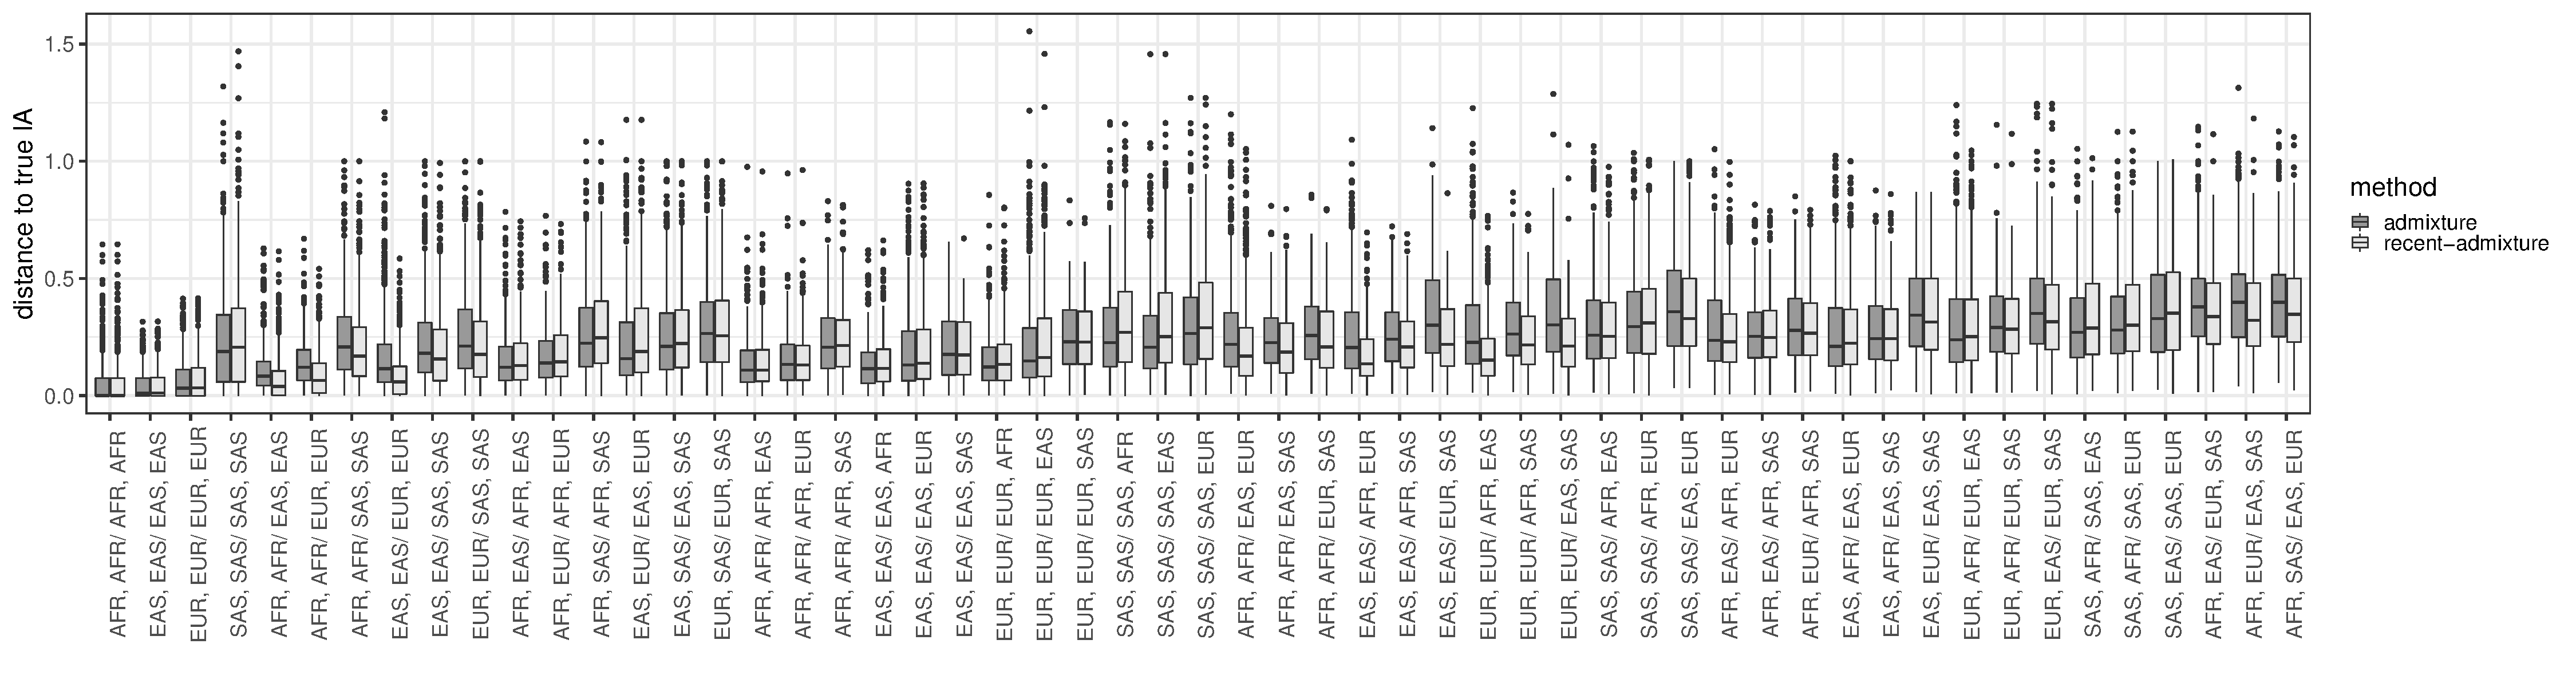
\includegraphics[width=\textwidth]{deviations_mixed_allcases.pdf}
  \caption{For all cases of second generation admixed individuals, we
    compare estimation accuracy of IA using the EUROFORGEN AIMset.}
  \label{fig:mixed_allcases}
\end{sidewaysfigure}

\begin{figure*}[htb]
  \hspace{3cm} (A) \hspace{8cm} (B)
  \begin{center}
    \parbox[b]{0.45\textwidth}{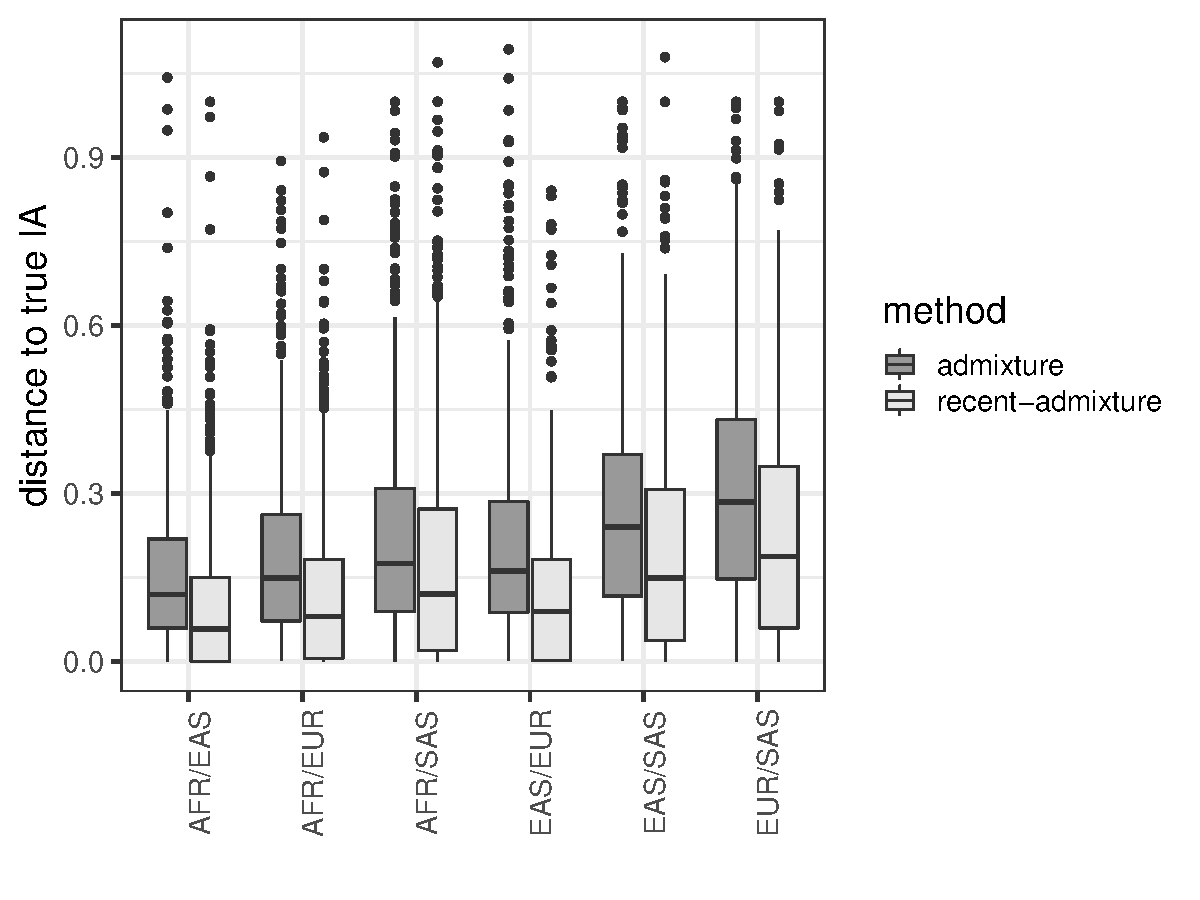
\includegraphics[width=0.45\textwidth]{deviations_mixed_Kidd.pdf}\vspace{2cm}}
    \hspace{1cm}
    \parbox[b]{0.45\textwidth}{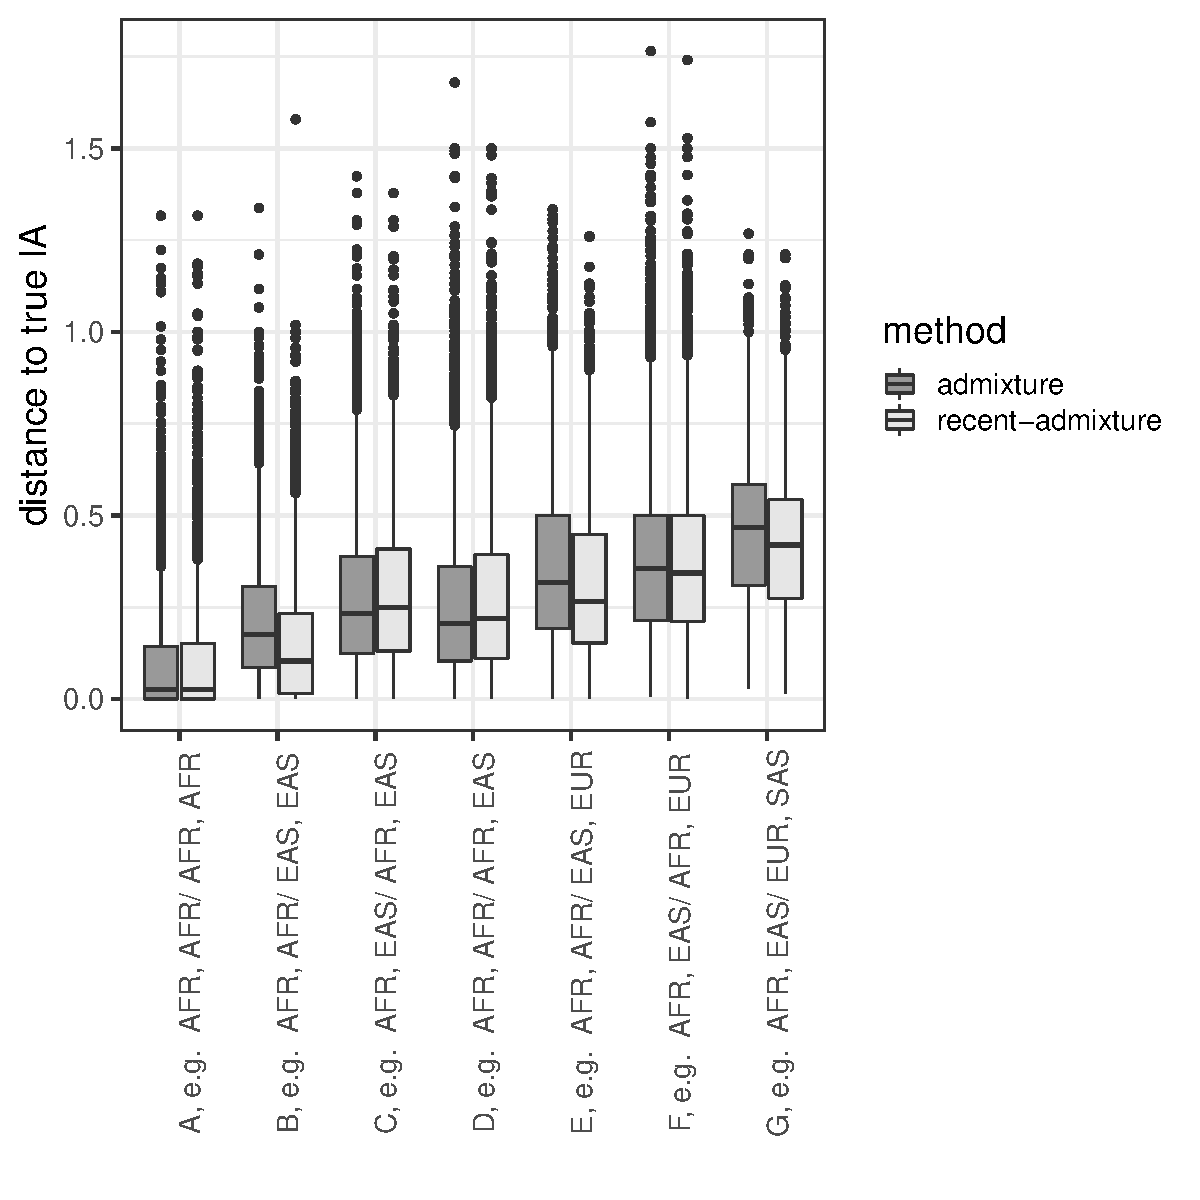
\includegraphics[width=0.45\textwidth]{deviations_mixed_cases_Kidd.pdf}}
  \end{center}
  \caption{\label{fig:mixed_cases_Kidd} Same as in
    Figure~\ref{fig:mixed_cases}, but using the Kidd AIMset.}
\end{figure*}

\begin{sidewaysfigure}
  \centering
  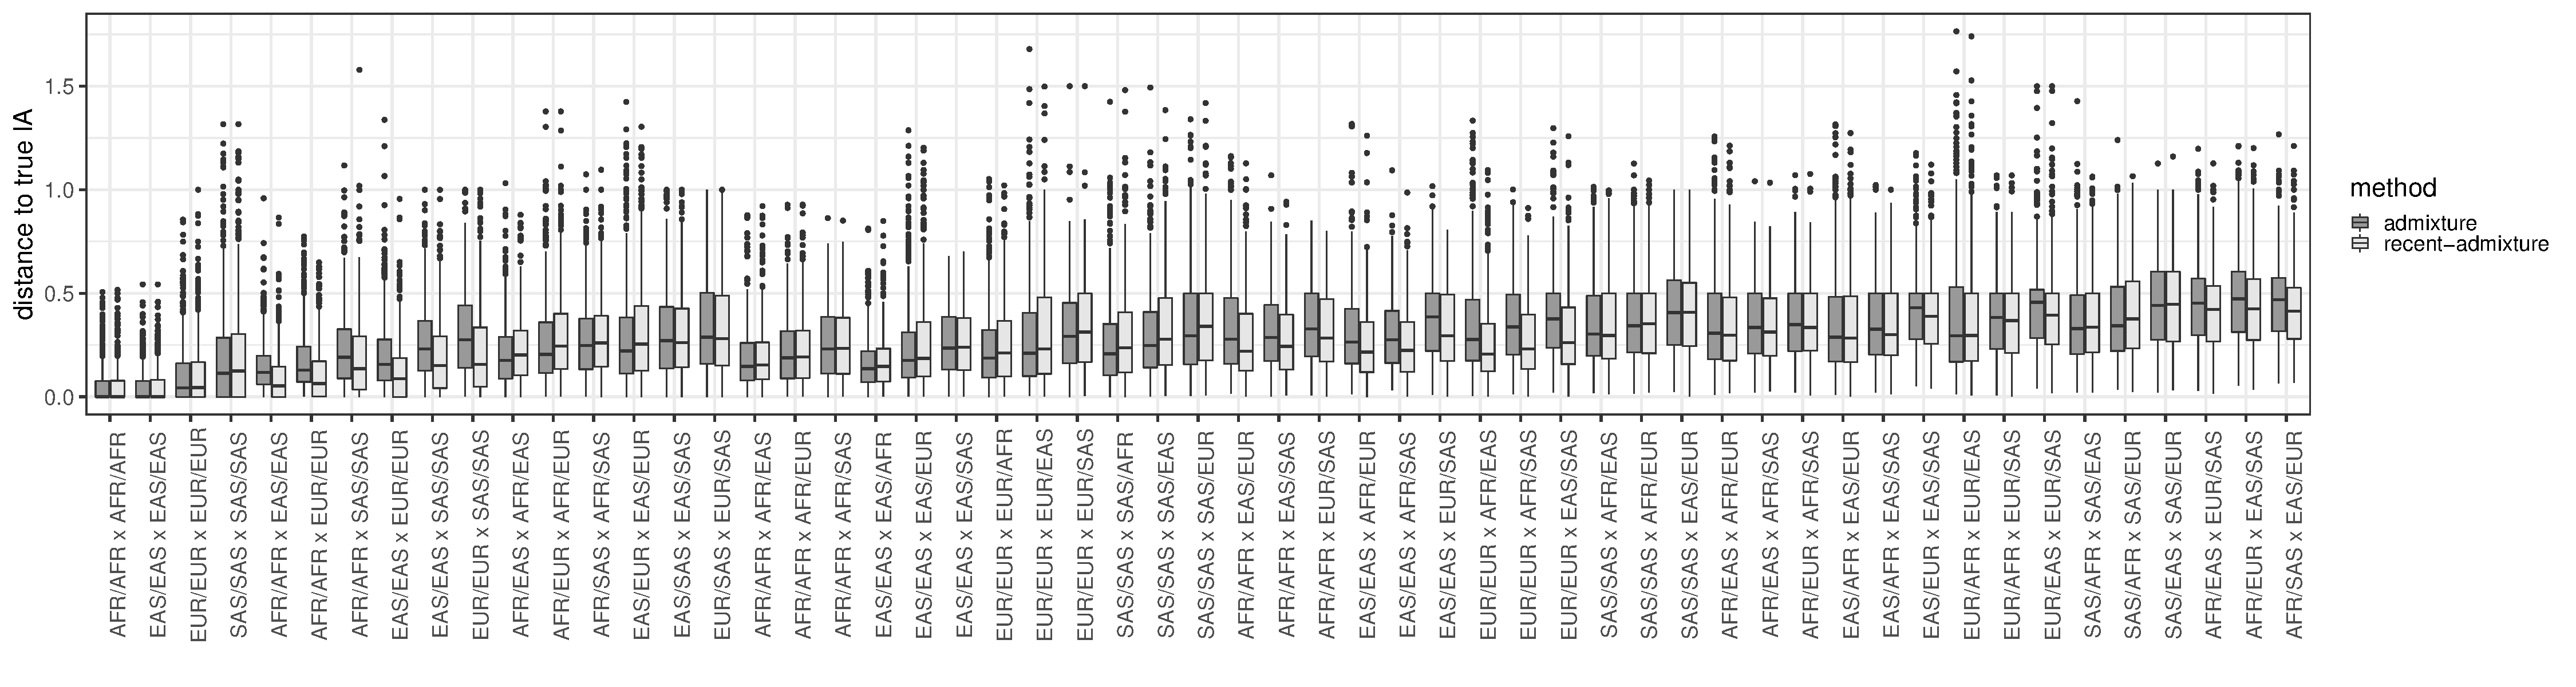
\includegraphics[width=\textwidth]{deviations_mixed_allcases_Kidd.pdf}
  \caption{Same as in Figure~\ref{fig:mixed_allcases}, but using the
    Kidd AIMset.}
  \label{fig:mixed_allcases_Kidd}
\end{sidewaysfigure}

\begin{table}
  \centering
  \begin{tabular}{l|rrrrrr}
Case & B & C & D & E & F & G \\ \hline
AUC &  0.982  &  0.655  &  0.855  &  0.983  &  0.921  &  0.982 \\ Power at $p=0.01$ & 0.92  &  0.29  &  0.5  &  0.89  &  0.65  &  0.89 \\
 \end{tabular}

  \caption{Same as Table~\ref{tab:power}, but using the Kidd AIMset.}
  \label{tab:power_Kidd}
\end{table}

\begin{figure*}[htb]
  \begin{center}
    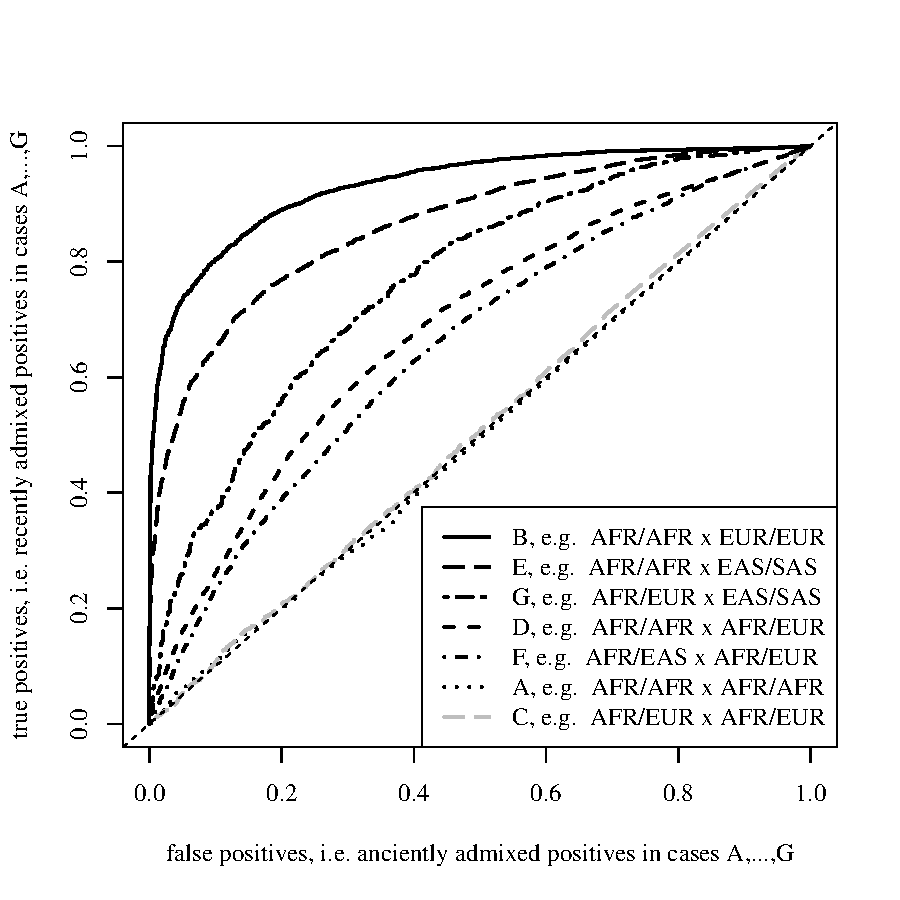
\includegraphics[width=0.45\textwidth]{roc-curve-Kidd.pdf}
  \end{center}
  \caption{Same as in Figure~\ref{fig:ROC}, but using the Kidd
    AIMset.}
  \label{fig:ROC_Kidd} 
\end{figure*}

\end{document}

